%%%%%%%%%%%%%%%%%%%%%%%%%%%%%%%%%%%%%%%%%%%%%%%%%%%%%%%%%%%%%%%%%%%%%%%%%%%%%%%%
% AMS Beamer series / Bologna FC / Template
% Andrea Omicini
% Alma Mater Studiorum - Università di Bologna
% mailto:andrea.omicini@unibo.it
%%%%%%%%%%%%%%%%%%%%%%%%%%%%%%%%%%%%%%%%%%%%%%%%%%%%%%%%%%%%%%%%%%%%%%%%%%%%%%%%
%\documentclass[handout]{beamer}\mode<handout>{\usetheme{default}}
%
\documentclass[presentation, 10pt]{beamer}\mode<presentation>{\usetheme{AMSBolognaFC}}
%\documentclass[handout]{beamer}\mode<handout>{\usetheme{AMSBolognaFC}}
%%%%%%%%%%%%%%%%%%%%%%%%%%%%%%%%%%%%%%%%%%%%%%%%%%%%%%%%%%%%%%%%%%%%%%%%%%%%%%%%

%\usepackage{lmodern}
\usefonttheme{professionalfonts}
\usepackage{arev}
\usepackage{multicol}
\usepackage{wasysym}
\usepackage{amsmath,blkarray}
\usepackage{centernot}
\usepackage{fontawesome}
\usepackage{fancyvrb}
\usepackage[ddmmyyyy]{datetime}
\renewcommand{\dateseparator}{}
%\renewcommand{\thefootnote}{\fnsymbol{footnote}}
\newcommand{\version}{1}
\usepackage{biblatex}
	\makeatletter

\addbibresource{biblio.bib}
%%%%%%%%%%%%%%%%%%%%%%%%%%%%%%%%%%%%%%%%%%%%%%%%%%%%%%%%%%%%%%%%%%%%%%%%%%%%%%%%
\title[Leveraging LLMs in Software Engineering]
{Leveraging Large Language Models in Software Engineering}
%
\subtitle[Research, Prospectives, Concerns]
{Research, Perspectives, Concerns}
%
\author[\sspeaker{Aguzzi}]
{\speaker{Gianluca Aguzzi} \href{mailto:gianluca.aguzzi@unibo.it}{gianluca.aguzzi@unibo.it}}
%
\institute[DISI, Univ.\ Bologna]
{Dipartimento di Informatica -- Scienza e Ingegneria (DISI)\\\textsc{Alma Mater Studiorum} -- Universit{\`a} di Bologna}
%
\renewcommand{\dateseparator}{/}
\date[\today]{\today}
%
%%%%%%%%%%%%%%%%%%%%%%%%%%%%%%%%%%%%%%%%%%%%%%%%%%%%%%%%%%%%%%%%%%%%%%%%%%%%%%%%
\begin{document}

\nocite{*}
%%%%%%%%%%%%%%%%%%%%%%%%%%%%%%%%%%%%%%%%%%%%%%%%%%%%%%%%%%%%%%%%%%%%%%%%%%%%%%%%

%/////////
\frame{\titlepage}
%/////////
%% print toc
\begin{frame}{Outline}
	\tableofcontents
\end{frame}
%===============================================================================

\section{Introduction to LLMs}
\begin{frame}{Today Lesson in a Nutshell}
	\centering
	
\includegraphics[width=0.5\textwidth]{img/meme.jpg}
\end{frame}
\begin{frame}[plain]
\centering
\huge{
	\textbf{Natural Language Processing} (NLP)
}
\\[1em]
\large{
	{A subfield of artificial intelligence that focuses \emph{understanding}, \emph{interpreting}, and \emph{generating} human language.}
}

\vspace{1em}
\small{
	\textbf{Resources}
	\begin{itemize}
		\item \url{https://github.com/keon/awesome-nlp?tab=readme-ov-file}
		\item \url{https://github.com/brianspiering/awesome-dl4nlp}
		\item \url{https://nlpprogress.com/}
		\item \url{https://www.unibo.it/it/studiare/dottorati-master-specializzazioni-e-altra-formazione/insegnamenti/insegnamento/2023/412644}
	\end{itemize}	
	
}
\end{frame}

\begin{frame}{Natural Language Processing}
	\begin{alertblock}{Goal}
		Identify the structure and meaning of \emph{words}, \emph{phases}, and \emph{sentences} in order to enable computers to understand and generate human language.
	\end{alertblock}
	\begin{exampleblock}{Why?}
		Improve \emph{human-computer} interaction, closing the gap between \emph{human communication} and \emph{computer understanding}.
	\end{exampleblock}
	\begin{alertblock}{Applications \textbf{(all around us)}}
		\begin{multicols}{2}
			\begin{itemize}
				\item \emph{Chatbots}
				\item \emph{Machine Translation}
				\item \emph{Speech Recognition}
				\item \emph{Sentiment Analysis}
				\item \emph{Question Answering}
				\item \emph{Code Generation}
			\end{itemize}
		\end{multicols}
	\end{alertblock}
\end{frame}
\begin{frame}{Natural Language Processing}
    \begin{alertblock}{Challenges}
        \begin{itemize}
            \item \textbf{Ambiguity:} Multiple meanings for words/phrases.
            \item \textbf{Context:} Meaning shifts with context (linguistic, cultural).
            \item \textbf{Syntax:} Sentence structure affects meaning.
            \item \textbf{Sarcasm/Idioms:} Non-literal language interpretation.
        \end{itemize}
    \end{alertblock}
    \begin{exampleblock}{Approaches}
        \begin{itemize}
            \item \textbf{Rule-Based:} Hand-crafted linguistic rules (e.g., \href{https://en.wikipedia.org/wiki/Georgetown-IBM\_experiment}{Georgetown–IBM}).
            \item \textbf{Statistical:} Probabilistic language modelling (e.g., hidden Markov model~\cite{DBLP:journals/coling/Merialdo94}).
            \item \textbf{ML/Deep Learning:} Algorithms learn from data; neural networks model complex patterns (RNN~\cite{DBLP:journals/corr/0001KYS17}, LSTM~\cite{DBLP:journals/neco/HochreiterS97}, GRU~\cite{DBLP:conf/mwscas/DeyS17}).
            \item[\faArrowRight] we will focus on \emph{\textbf{language models}}.
        \end{itemize}
    \end{exampleblock}
\end{frame}

\begin{frame}[plain]
	\centering
	\huge{
		What is a \textbf{Language Model}?
	}
	\\[1em]
	\large{
		{A \emph{machine learning} model that aims to predict and generate plausible text.}
	}
\end{frame}
\begin{frame}{Language Models}
	\begin{exampleblock}{Idea}
		text is a sequence of words, and language models learn the \emph{probability} of a word given the previous words.
	\end{exampleblock}
	\begin{exampleblock}{Example}
		\begin{itemize}
			\item \emph{The cat is on the <*>}
			\item \emph{The cat is on the \textbf{mat}.}
			\item \emph{The cat is on the \textbf{table}.}
		\end{itemize}
	\end{exampleblock}
	\begin{alertblock}{Tasks}
		\begin{itemize}
			\item \emph{Prediction:} Given a sequence of words, predict the next word (e.g., autocomplete).
			\item \emph{Classification:} Given a sequence of words, classify the text (e.g., sentiment analysis).
		\end{itemize}
	\end{alertblock}
\end{frame}
\begin{frame}{Language Models -- Phases}
    \begin{enumerate}
        \item \textbf{Tokenization}: split text into words, phrases, symbols, etc. \\
        \begin{itemize}
			\item \textit{Example:} "Hello, world!" $\rightarrow$ ["Hello", ",", "world", "!"]
		\end{itemize}
        \item \textbf{Embedding}: convert words into numerical vectors.
        \begin{itemize}
			\item \textit{Example:} "Hello" $\rightarrow$ [0.25, -0.75, 0.5, 1.0]
			\item it is possible to used pretrained embeddings (e.g., Word2Vec,  BERT).
		\end{itemize}
        \item \textbf{Modelling}: learn the probability of a word given the previous words.
        \begin{itemize}
			\item \textit{Example:} P("world" | "Hello,") $\rightarrow$ 0.8
		\end{itemize}
        \item \textbf{Generation/Classification}: use the model to generate text or classify it. \\
        \begin{itemize}
			\item \textit{Example for Generation:} Input: "The weather is" $\rightarrow$ Output: "sunny." \\
			\item     \textit{Example for Classification:} Input: "This is a spam email." $\rightarrow$ Output: Spam
     
		\end{itemize}
    \end{enumerate}
\textbf{Note:} each NLP solution can use different techniques for each phase.
\end{frame}
\begin{frame}[fragile]{Language Models -- Recurrent Neural Networks}

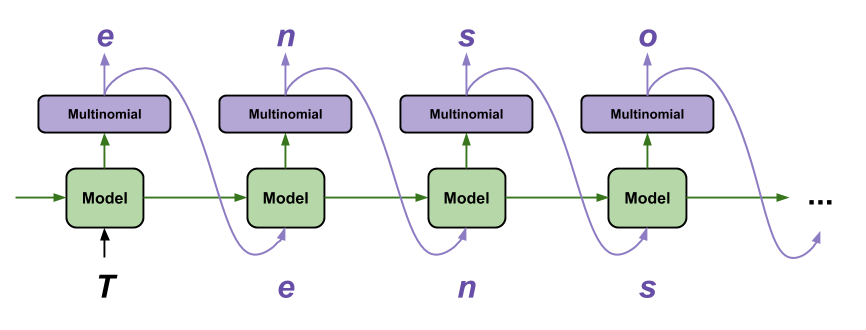
\includegraphics[width=\textwidth]{img/text-generation.png}

\end{frame}

\begin{frame}{Language Models -- Convolutional Networks}

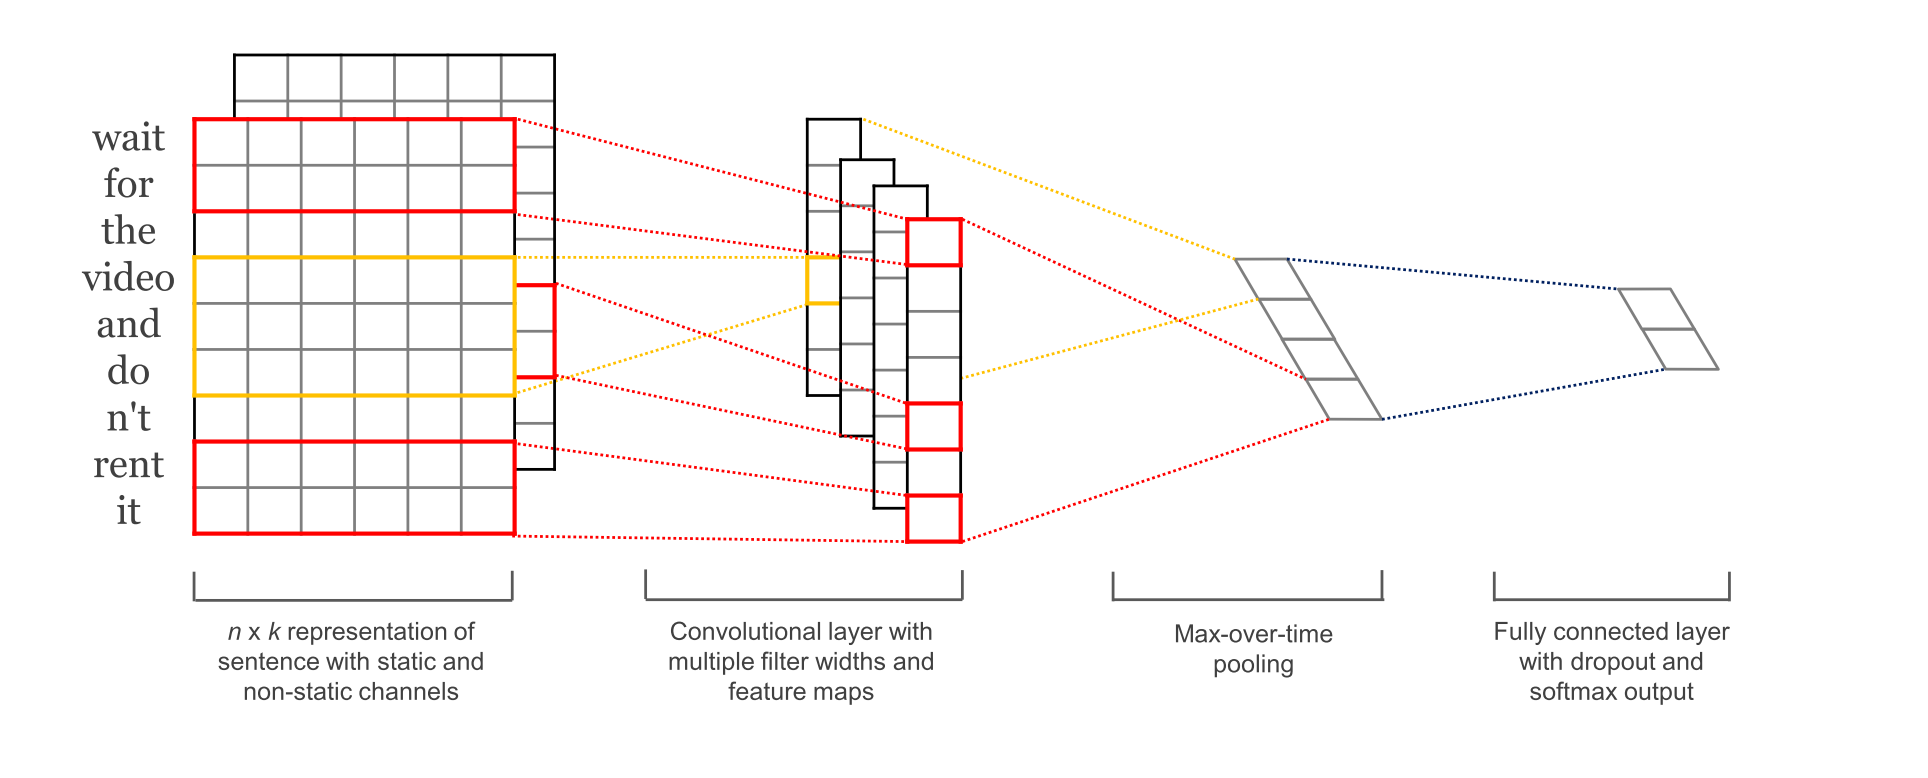
\includegraphics[width=\textwidth]{img/cnn-text.png}

\end{frame}

\begin{frame}{RNN and CNN -- Limitations}
\begin{itemize}
	\item \textbf{RNN:} long-term dependencies are hard to capture.
	\item \textbf{RNN:} slow to train; not suitable for large-scale data.
	\item \textbf{CNN:} fixed-size input window; not suitable for variable-length text
	\item \textbf{Both:} struggle with large-scale data.
	\item \textbf{Solution:} \emph{Multi-head attention}: that is the core of \emph{transformers}.
\end{itemize}
\end{frame}
\begin{frame}{Language Models -- Transformers~\cite{DBLP:conf/nips/VaswaniSPUJGKP17}}
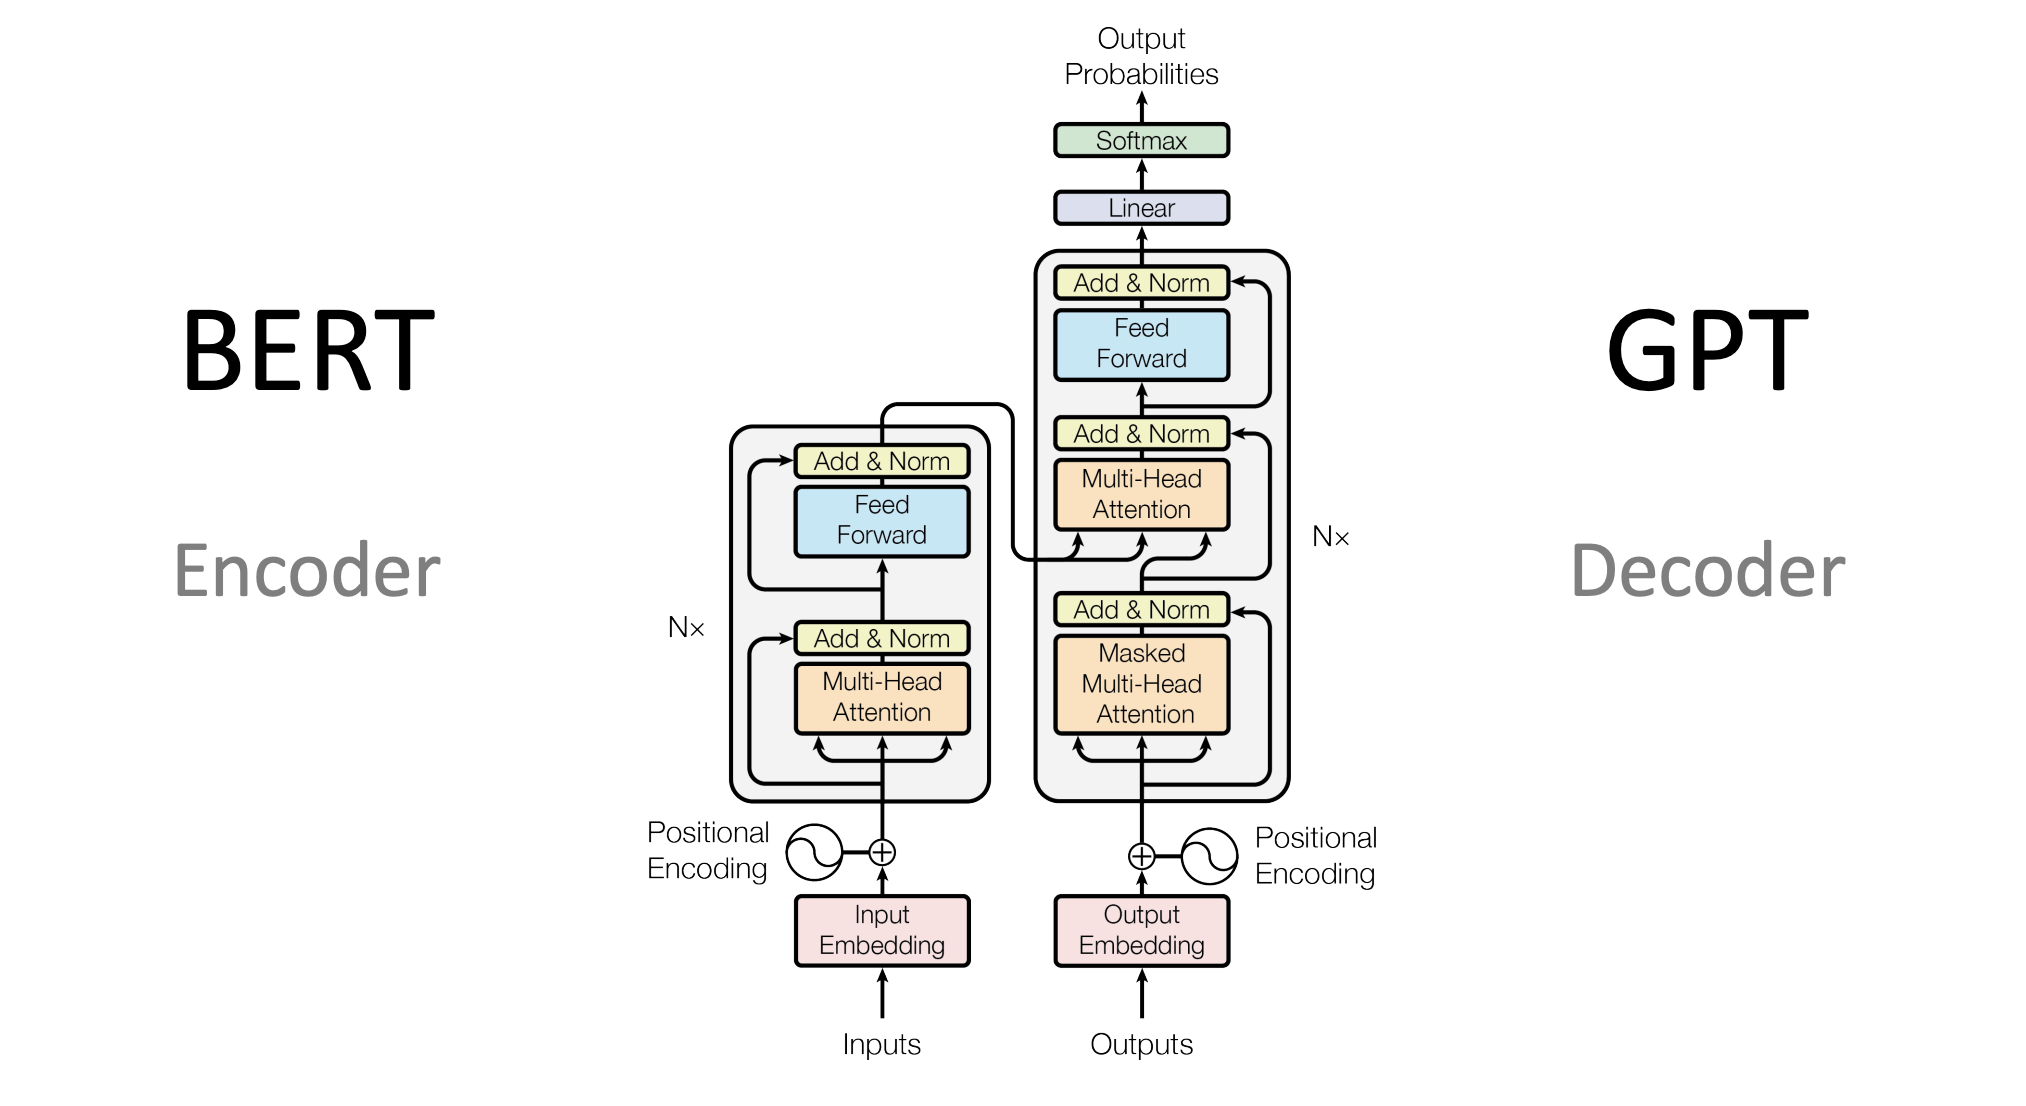
\includegraphics[width=\textwidth]{img/transformers.png}
\centering{
\url{https://www.youtube.com/watch?v=4Bdc55j80l8}
\url{https://www.youtube.com/watch?v=SZorAJ4I-sA}

}
\end{frame}

\begin{frame}[plain]
	\huge{
		\textbf{Large Language Model} (LLM)
	}\\[1em]
	\large{
		{A \emph{language model} with a \emph{large} number of parameters, trained on a \emph{large} corpus of text.}
	}
\end{frame}

\begin{frame}{LLM -- Implementation Strategies}
    \begin{itemize}
        \item \textbf{Transformers} as the foundational architecture, characterized by:
        \begin{itemize}
            \item Long-range context (\emph{Attention})
            \item Efficient large-scale training (\emph{Parallelization})
            \item Model growth (\emph{Scalability})
        \end{itemize}
        \item \textbf{Pretraining:} Involves training the model on a vast corpus of text to learn a wide range of language patterns and structures.
        \item \textbf{Fine-tuning:} Refines the pretrained model for specific tasks, enhancing its applicability and performance on targeted applications.
    \end{itemize}
\end{frame}

\begin{frame}{LLM -- Training Paradigms}
\textbf{The Learning Cake:} An analogy to describe the layered approach in training methodologies.
\begin{itemize}
    \item \textbf{Self-supervised Learning:} Models learn patterns from unlabelled data, reducing the need for expensive annotations. Ideal for initial \emph{understanding} of language structures.
    \item \textbf{Supervised Learning:} Enhances accuracy with labeled data, crucial for tasks requiring specific outcomes like \emph{classification} and \emph{translation}.
    \item \textbf{Reinforcement Learning:} Adapts through trial and error using rewards, fine-tuning decision-making skills in scenarios like \emph{dialogue generation}.
\end{itemize}
\end{frame}
\begin{frame}{LLM -- Paradigm Shift}
	\centering
	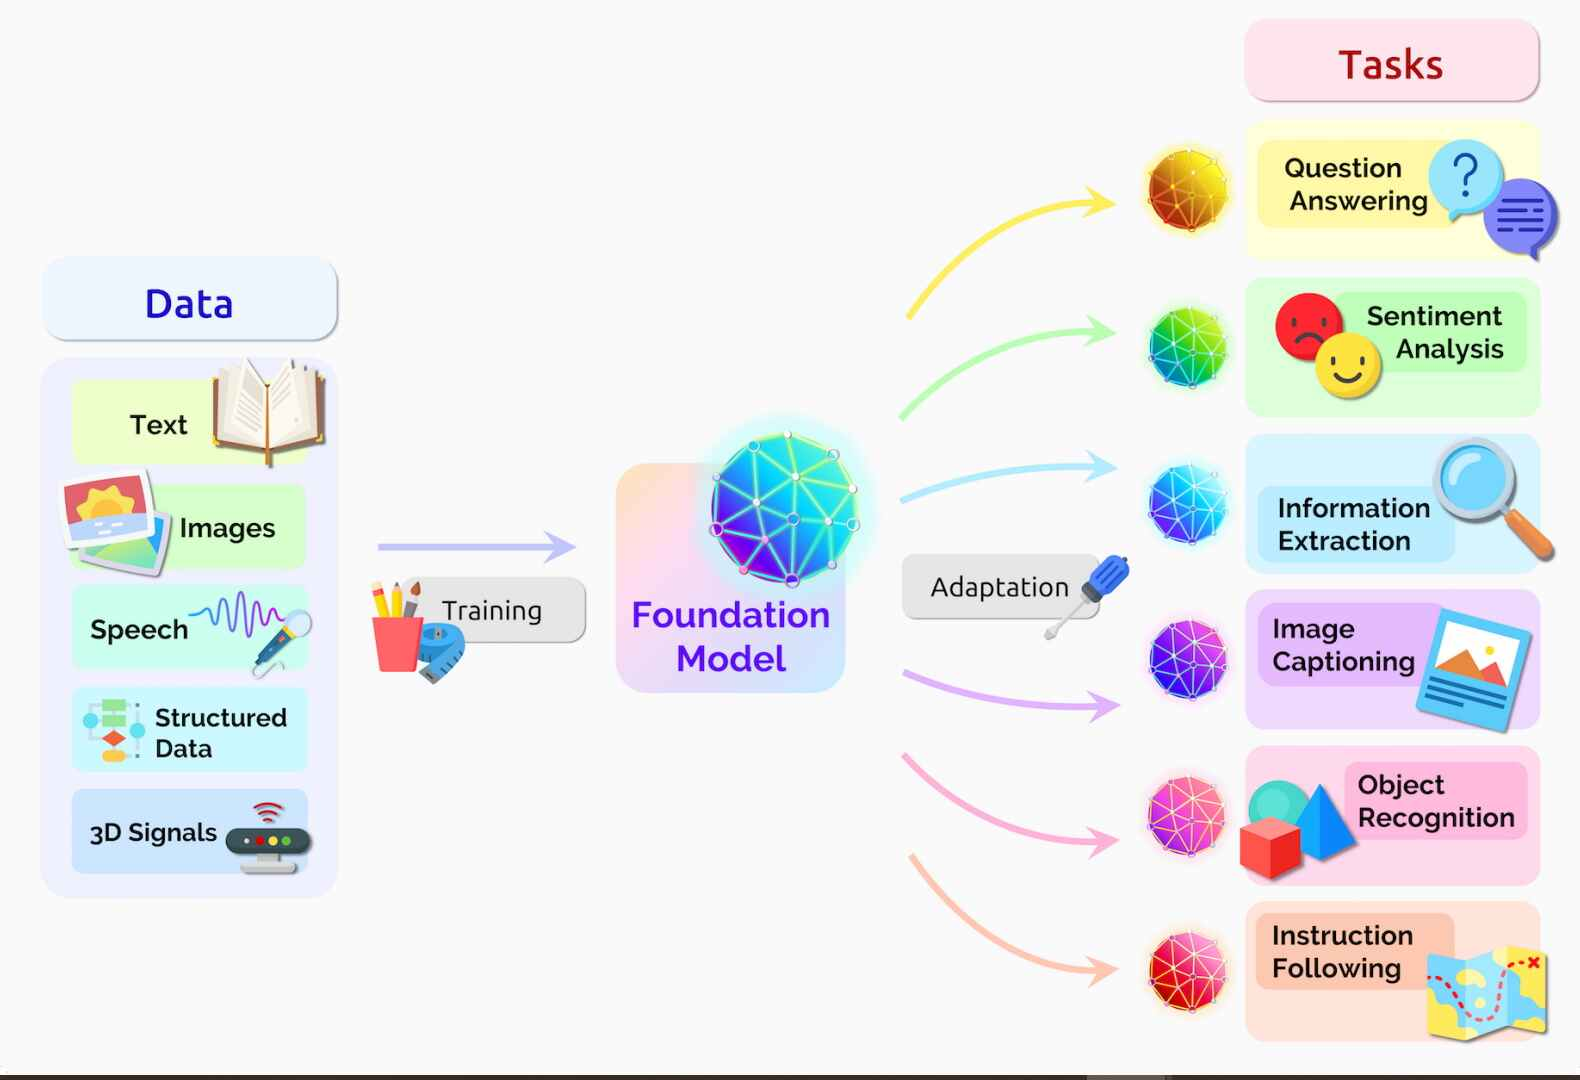
\includegraphics[height=7.5cm]{img/llm-idea.jpg}
\end{frame}
%\begin{frame}{LLM -- Adaptation}
%	\begin{itemize}
%			\item \textbf{Fine-tuning:} Adapt model to specific tasks through supervision.
			
%			\item \textbf{Prompting:} Guide model to specific outputs.
%			\begin{itemize}
%					\item \emph{Zero-shot learning:} Direct instruction for desired outcome without fine-tuning.
%					\item \emph{Few-shot learning:} Use minimal examples in prompt for in-context learning.
%					\begin{itemize}
%							\item \textbf{Example:} Summarization with few example summaries.
%							\item \textbf{RAG:} Retrieval-Augmented Generation for information-rich answers.
%					\end{itemize}
%					\item \emph{Chain-of-thought:} Break down problems into intermediate steps.
					%\item \emph{Analogical reasoning:} Solve by drawing parallels to known scenarios.
%					\item More examples will be shown in SE applications.
%			\end{itemize}
%	\end{itemize}
%	\end{frame}
\begin{frame}{LLM -- Scalability}
	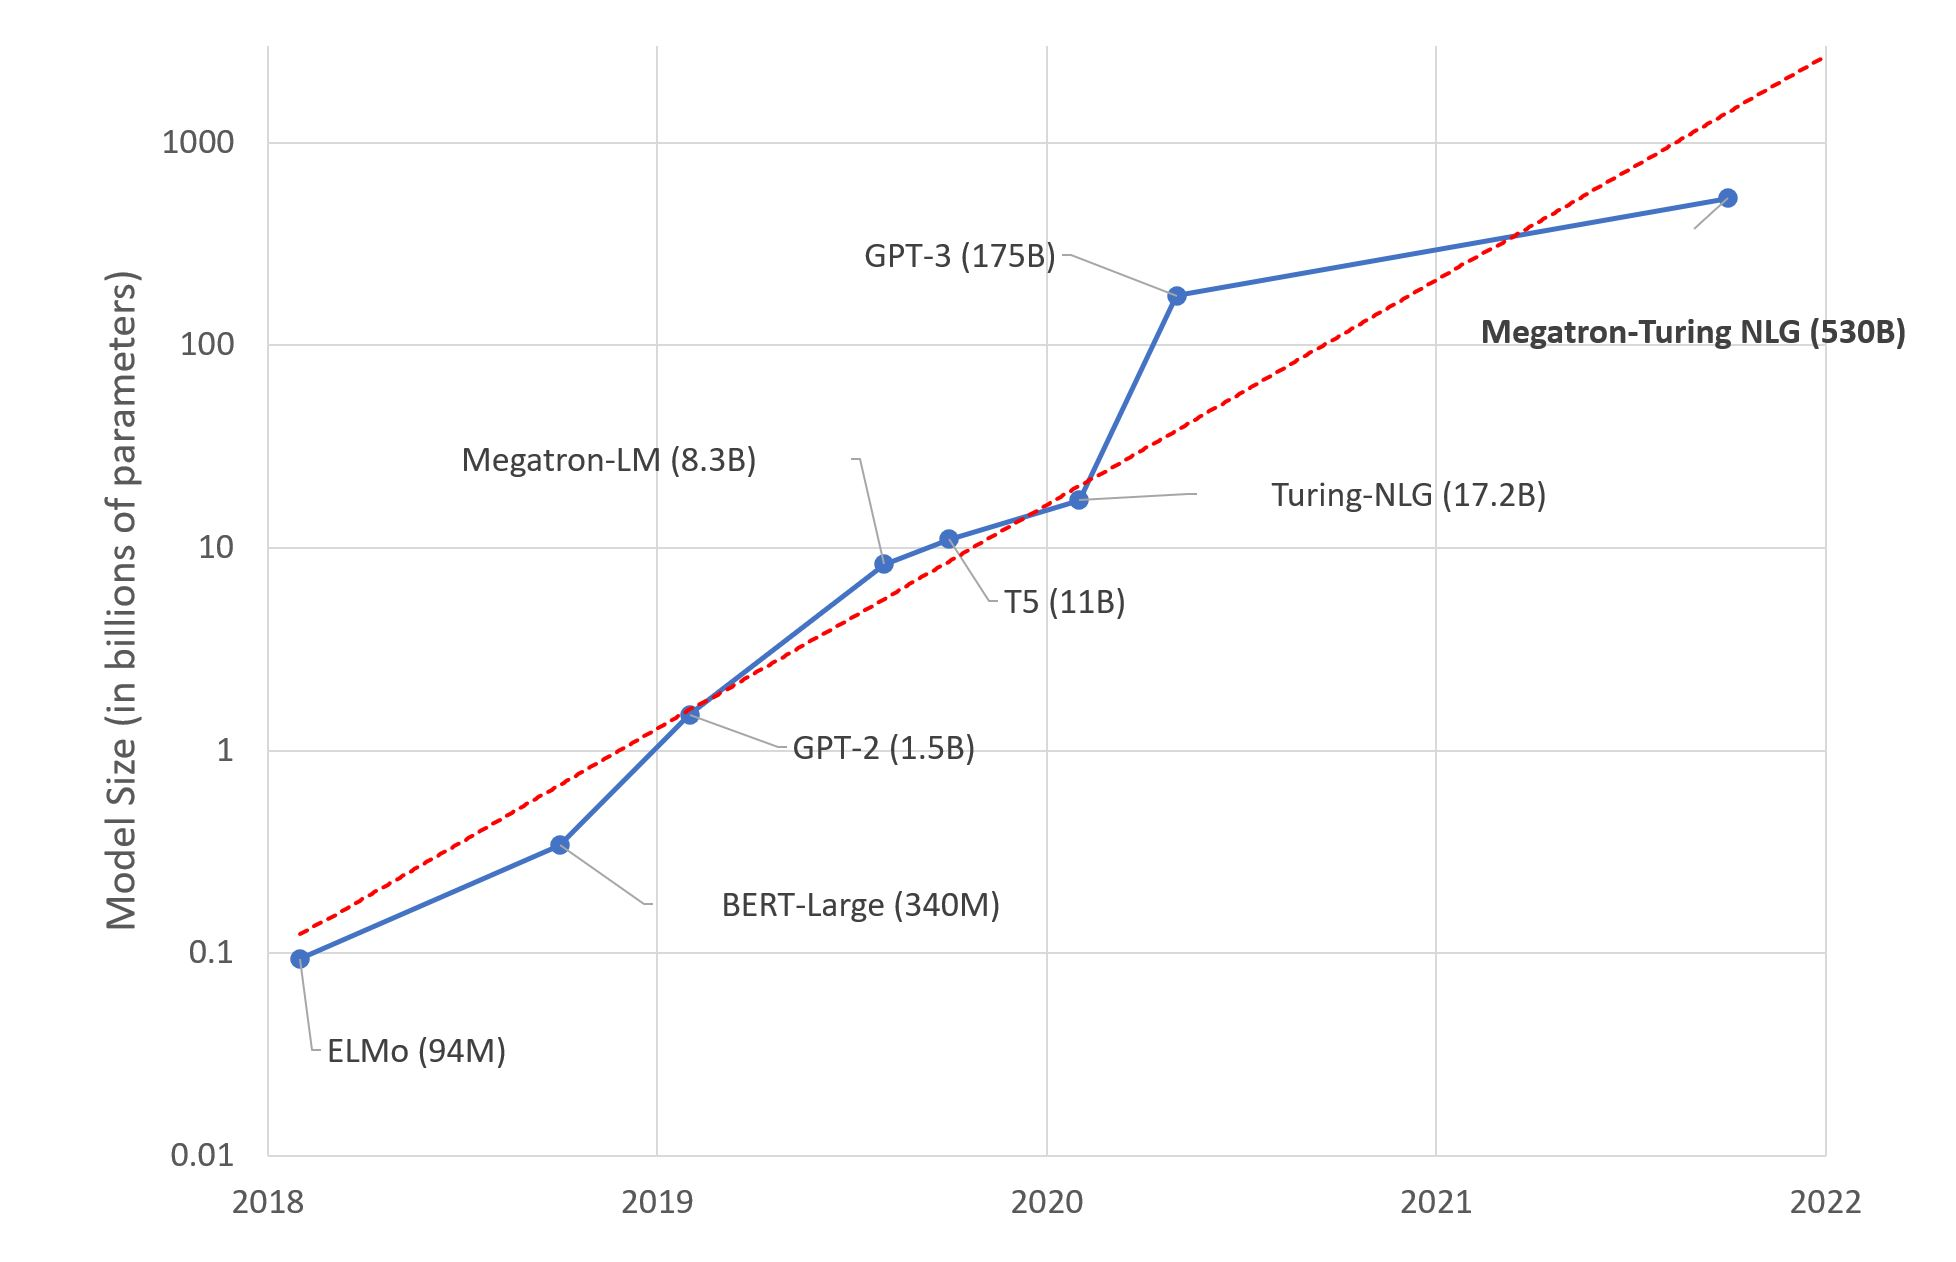
\includegraphics[width=\textwidth]{img/over-year.jpg}
\end{frame}
\begin{frame}{LLM -- Scalability}
	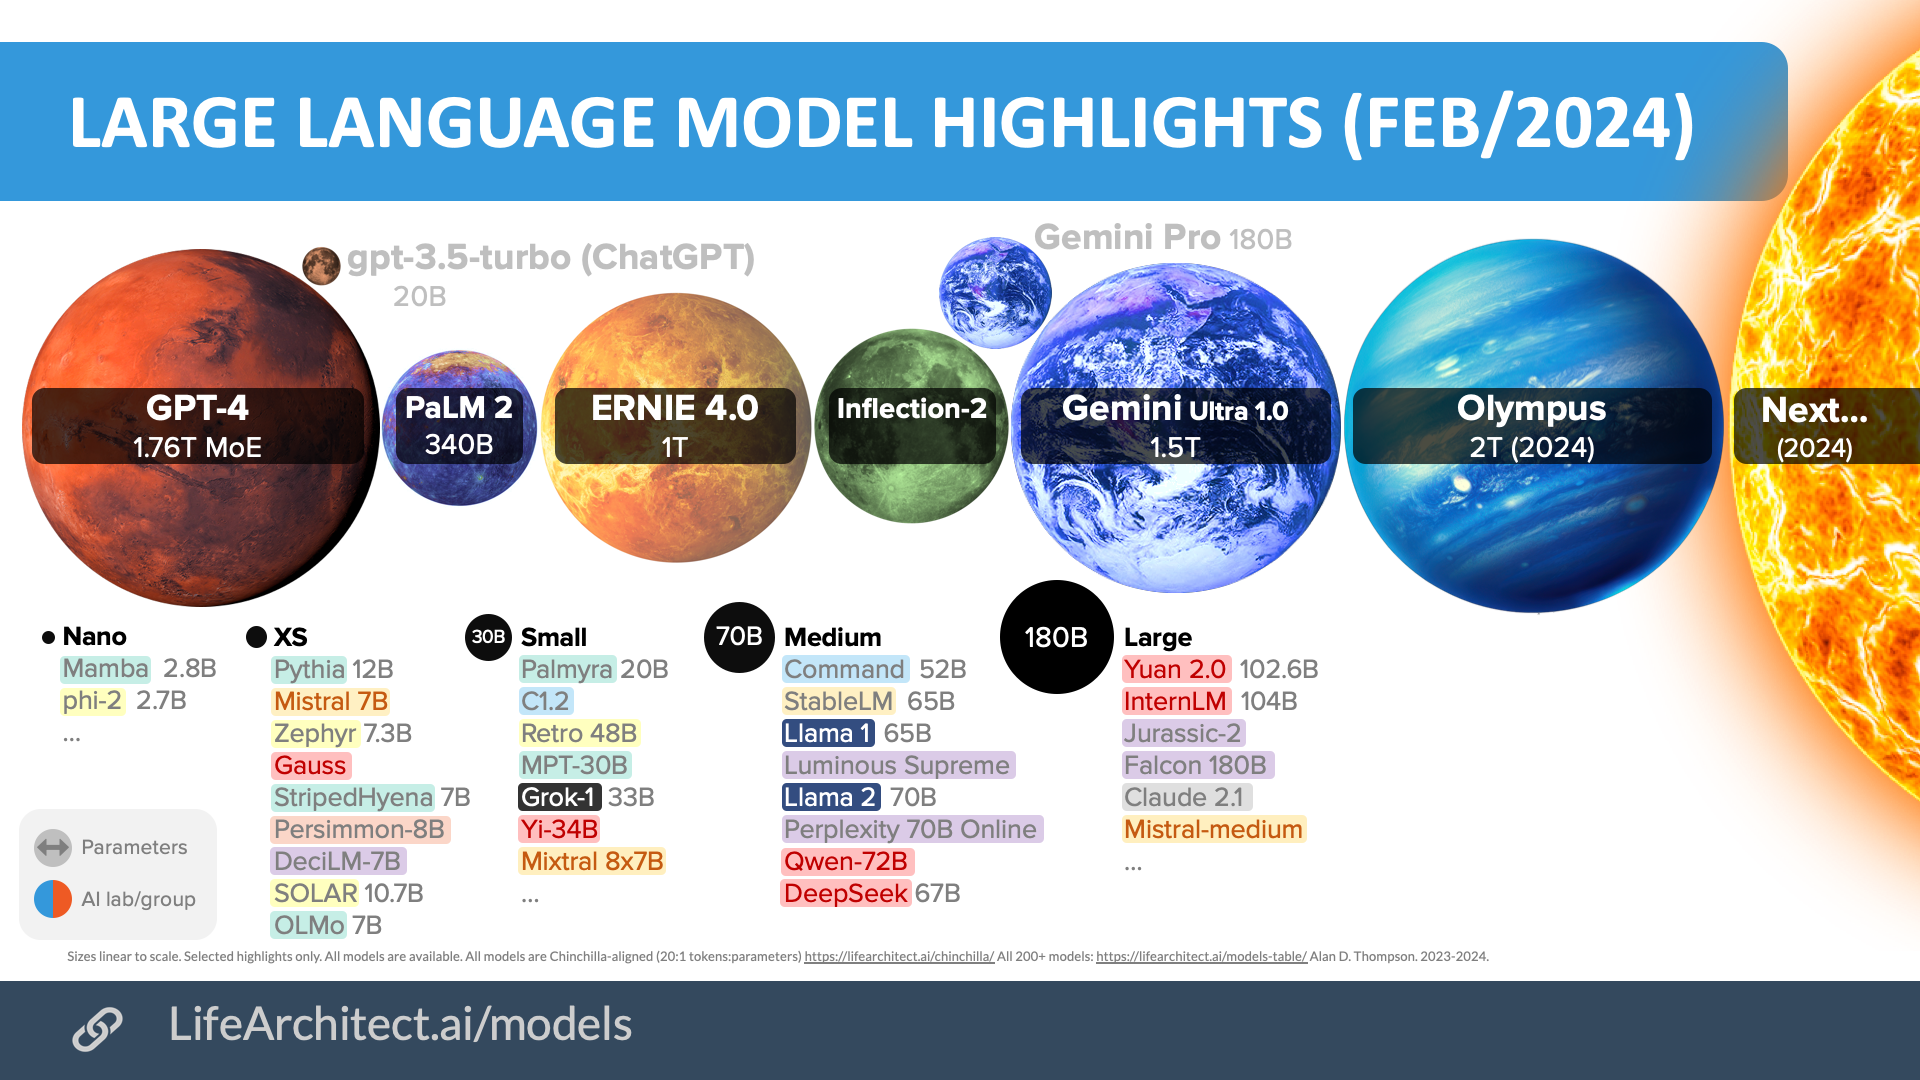
\includegraphics[width=\textwidth]{img/image-size.png}
\end{frame}
\begin{frame}{LLM -- Emergent Properties~\cite{DBLP:journals/tmlr/WeiTBRZBYBZMCHVLDF22}}
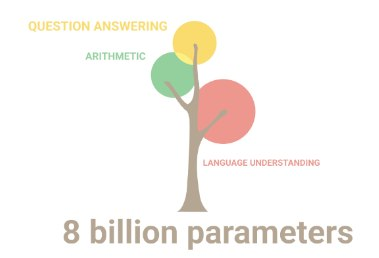
\includegraphics[width=0.35\textwidth]{img/small.jpg}
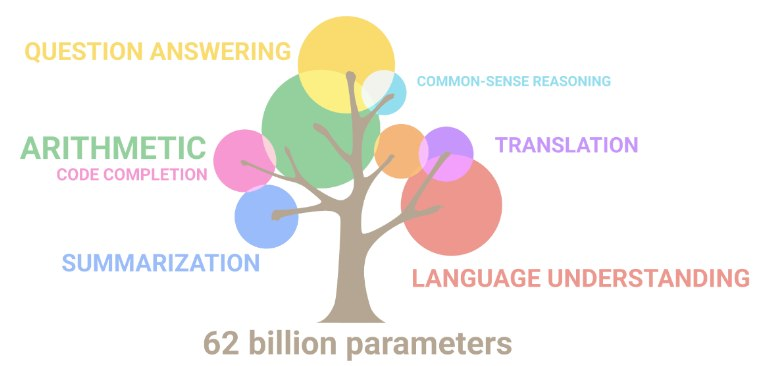
\includegraphics[width=0.55\textwidth]{img/medium.jpg}
\centering
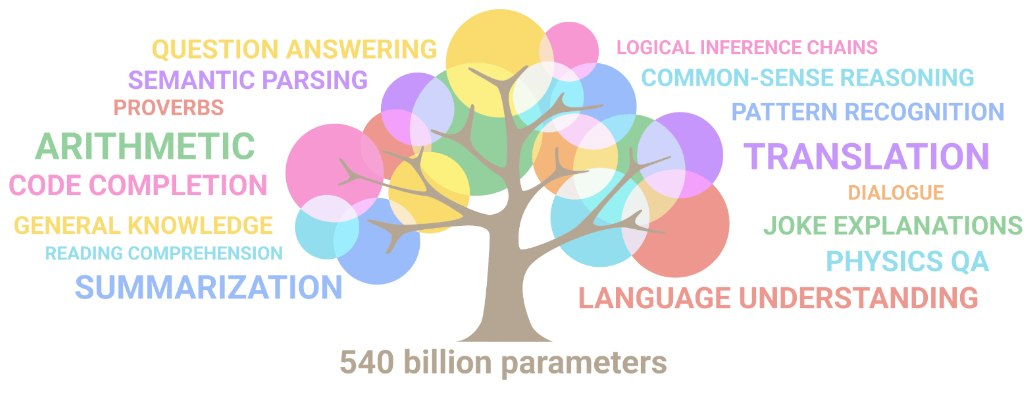
\includegraphics[width=0.8\textwidth]{img/big.jpg}
\end{frame}
\begin{frame}{LLM -- State-of-the-art foundational models}
	\begin{itemize}
		\item \textbf{GPT-4/3} \faLock: generative Pre-trained Transformer (OpenAI)
		\begin{itemize}
			\item State-of-the-art in \emph{language generation} and \emph{translation}.
			\item GPT-4 is multi-modal, capable of processing text, images, and audio.
		\end{itemize}
		\item \textbf{Gemini}\footnote{\url{https://gemini.google.com/app}} \faLock: most capable multi-modal model from Google.
		\item \textbf{Llama} (1/2)~\cite{touvron2023llama} \faUnlock: Large Language Model Meta AI (Meta) 
		\begin{itemize}
			\item One of the first open source LLMs with a relevant number of parameters.
		\end{itemize}
		\item \textbf{Mistral~\cite{jiang2023mistral}/Mixtral\footnote{\url{https://huggingface.co/docs/transformers/model_doc/mixtral}}/Falcon~\cite{almazrouei2023falcon}} \faUnlock: several completely open and transparent models from several companies. 
	\end{itemize}
\centering
More at: \url{https://lifearchitect.ai/models-table/}
\end{frame}
\begin{frame}{LLM applications: Chatbots\footnote{\url{https://openai.com/blog/chatgpt}}}
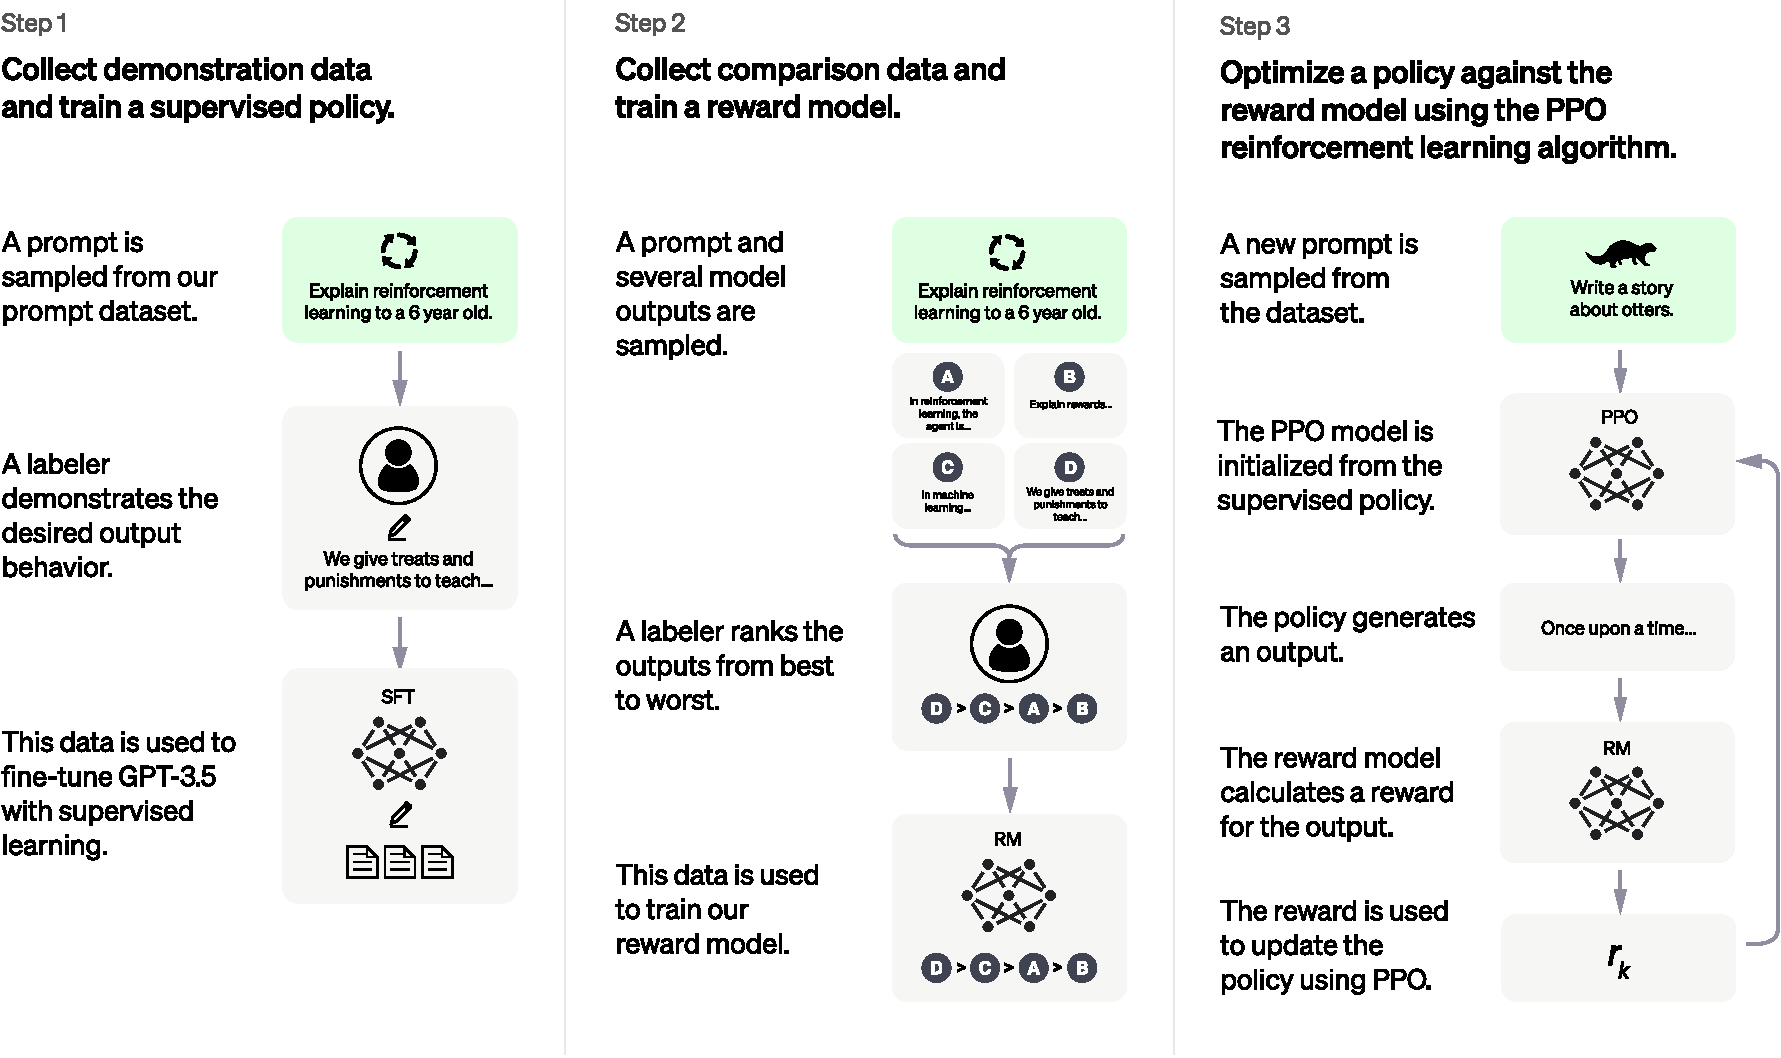
\includegraphics[width=\textwidth]{img/image.pdf}
\end{frame}
\begin{frame}{LLM applications: Medical Diagnosis\footnote{https://sites.research.google/med-palm/}}

\includegraphics[width=\textwidth]{img/palm-med.png}
\end{frame}
\begin{frame}{Robotics~\cite{DBLP:journals/corr/abs-2205-06175}}
	\centering
	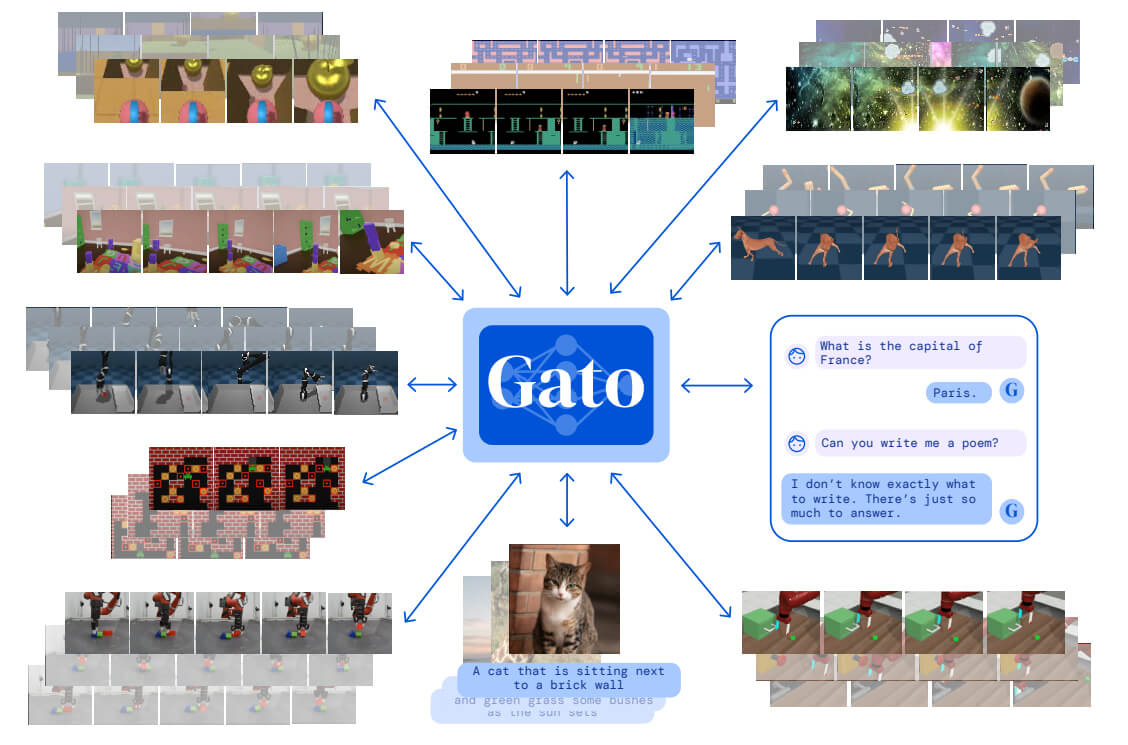
\includegraphics[width=0.9\textwidth]{img/generalistic-agent.jpeg}
\end{frame}
\begin{frame}{LLM Applications: Code Generation\footnote{\url{https://github.blog/2023-03-22-github-copilot-x-the-ai-powered-developer-experience/}}}
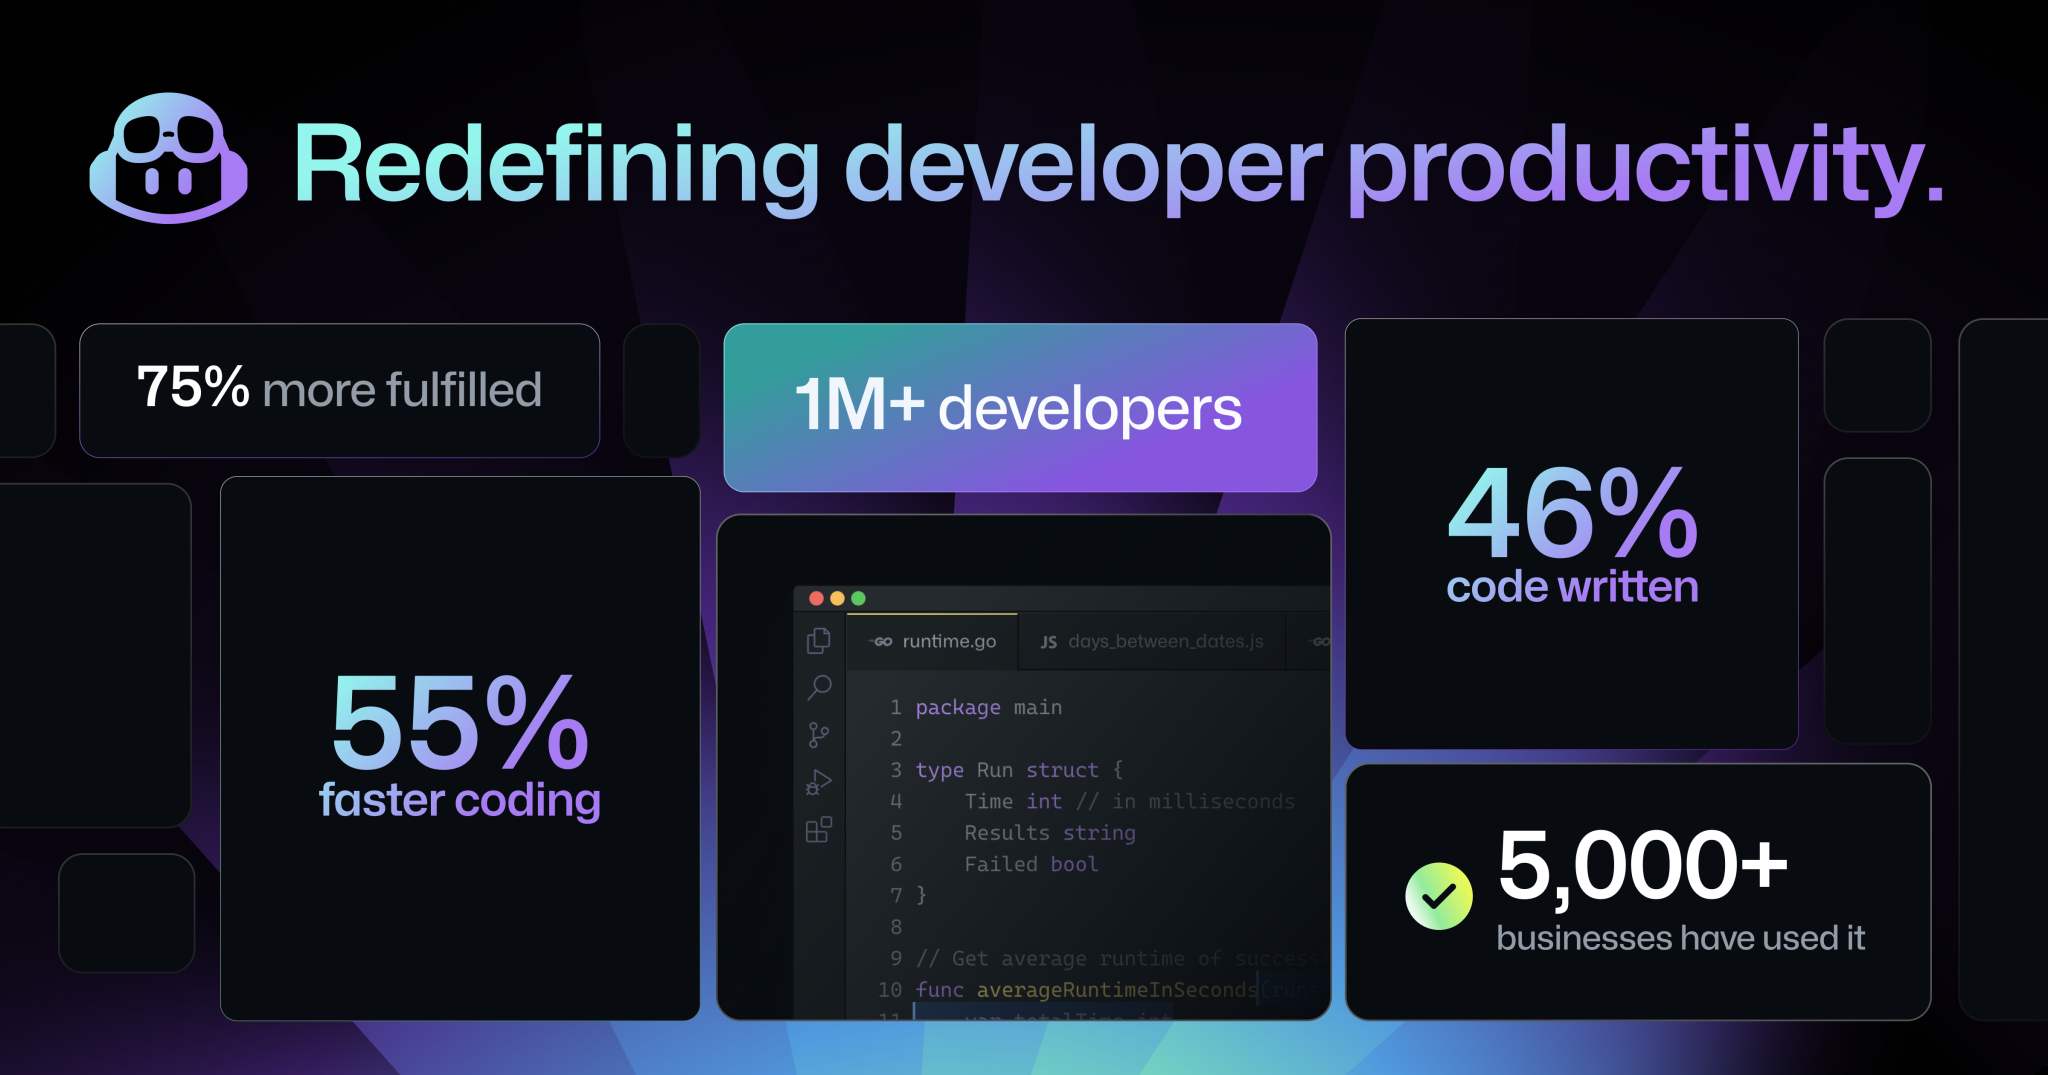
\includegraphics[width=\textwidth]{img/copilot.png}
\end{frame}
\begin{frame}{LLM Concerns -- Training Cost}
\centering
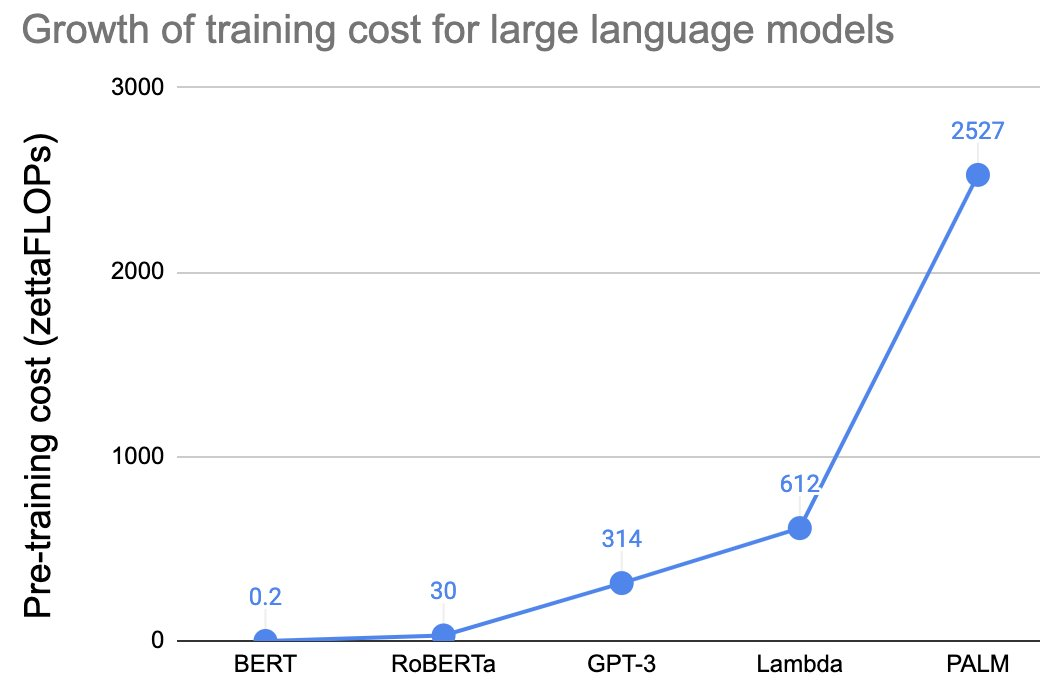
\includegraphics[width=0.8\textwidth]{img/training-cost.jpg}
\end{frame}
\begin{frame}{LLM Concerns -- Privacy}
	
\includegraphics[width=\textwidth]{img/italy-privacy-concern.png}
\end{frame}
\begin{frame}{LLM Concerns -- Hallucination}
\emph{Hallucination} is the generation of text that is not grounded in reality.
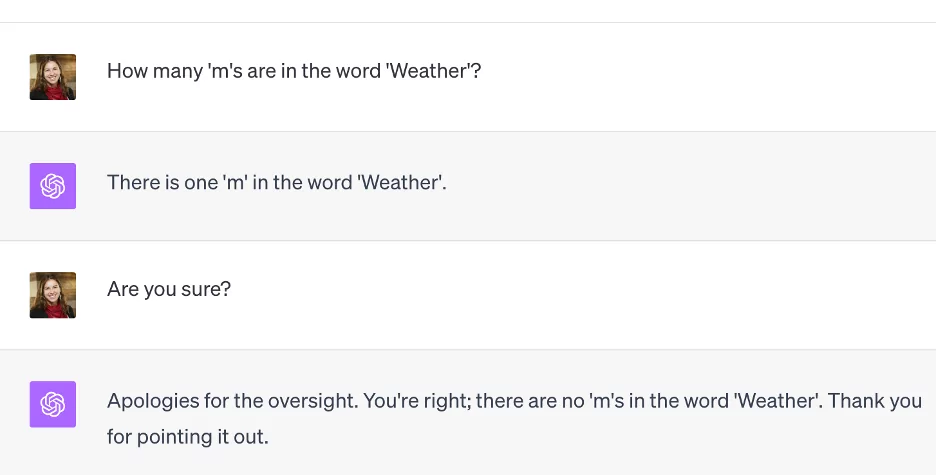
\includegraphics[width=\textwidth]{img/hallucinations.png}
\end{frame}
\section{Machine Learning for Software Engineering}
\begin{frame}[plain]
\centering
\huge{Machine Learning for Software Engineering}
\\[1em]
\large{
Application of machine learning \emph{techniques} and \emph{methodologies} to address challenges and solve problems in the field of software engineering}
\\[1em]
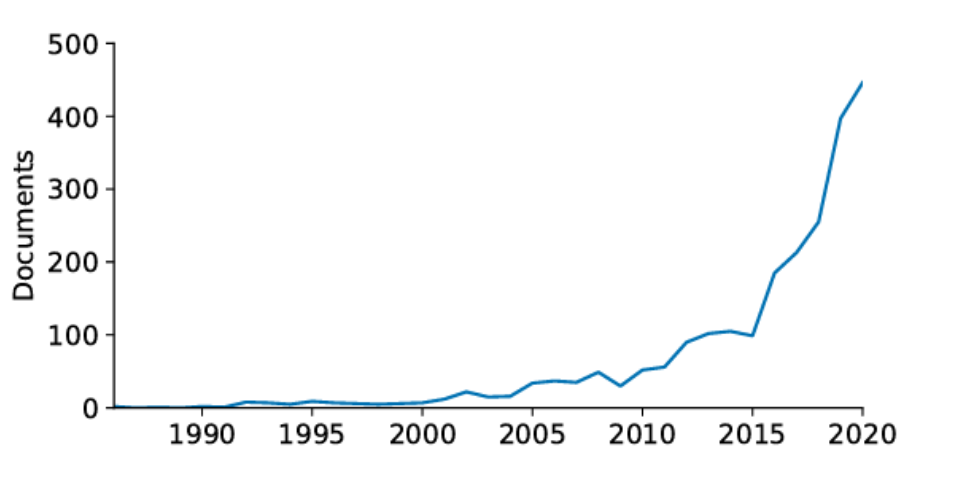
\includegraphics[width=0.7\textwidth]{img/pubblication-over-year.png}
\end{frame}
\begin{frame}{Machine Learning for Software Engineering}
\begin{exampleblock}{Why?}
	\begin{itemize}
	\item \textbf{Automation:} automate repetitive tasks (e.g., code generation).
	\item \textbf{Prediction:} predict software quality, bugs, and performance.
	\item \textbf{Optimization:} optimize software development processes.
	\item \textbf{Understanding:} understand software artifacts and processes.
	\item \textbf{Personalization:} personalize software development tools.
\end{itemize}
\end{exampleblock}
\begin{exampleblock}{When?}
	\begin{itemize}
		\item \textbf{Requirement Engineering:} requirements elicitation and analysis.
		\item \textbf{Design:} design patterns, architecture, and modeling.
		\item \textbf{Implementation:} code generation, refactoring, and bug fixing.
		\item \emph{\textbf{Testing:}} test case generation, fault prediction...
		\item \textbf{Maintenance:} bug prediction, code review...
	\end{itemize}
\end{exampleblock}
\end{frame}
\begin{frame}{Machine Learning for Software Engineering}
\begin{exampleblock}{How?~\cite{DBLP:journals/csur/KottiGS23}}
\centering
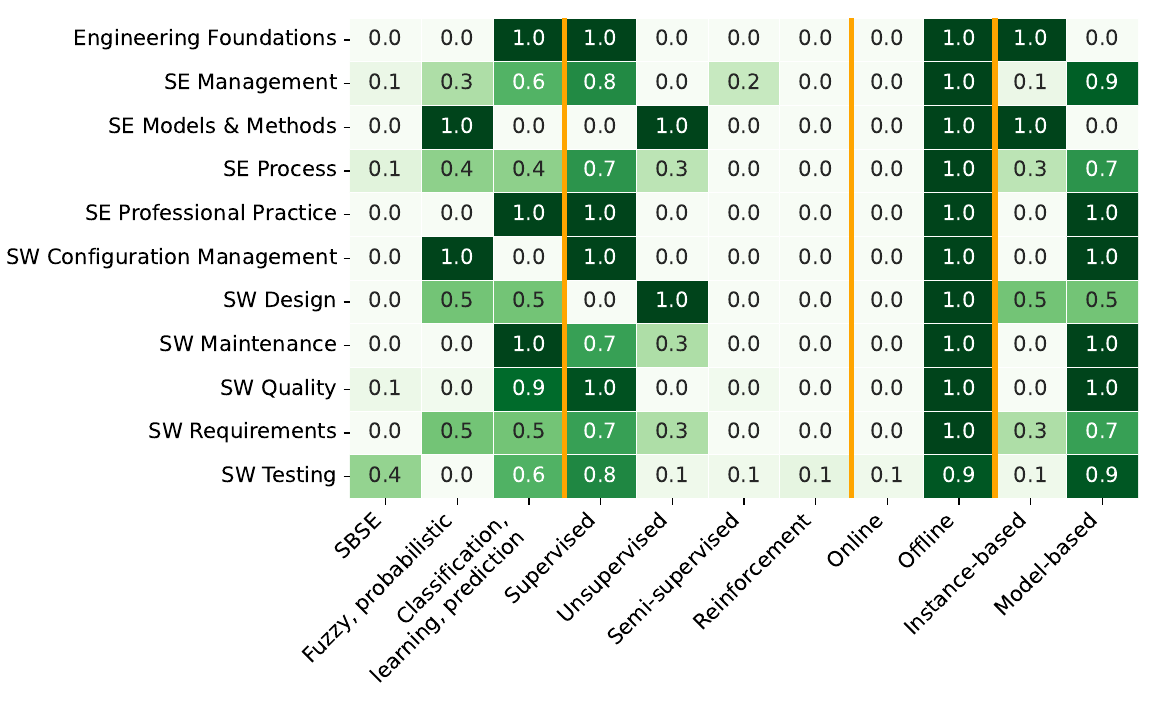
\includegraphics[width=0.9\textwidth]{img/distrubution.png}
\end{exampleblock}
\end{frame}
\begin{frame}{Early approaches -- Evolutionary Algorithms}
\begin{exampleblock}{What}
	Evolutionary algorithms are a \emph{family} of optimization algorithms inspired by the process of natural evolution
\end{exampleblock}
\begin{exampleblock}{Where}
	\begin{itemize}
		\item Program \emph{synthesis} / \emph{sketching}~\cite{lezama2008program} (programming the unpromgrammable) -- \emph{Genetic Programming}.
	
		\item \emph{Test case generation} -- evolve test cases to maximize coverage (mutation tests~\cite{DBLP:journals/infsof/Dominguez-JimenezEGM11}).
		\item \emph{Software Quality Prediction} -- understand and predict software quality~\cite{evett1998gp}
		\item Robotic design -- \emph{automatic design}~\cite{DBLP:journals/swarm/FrancescaBBTB14} of robots. 
	\end{itemize}
\end{exampleblock}
\end{frame}

\begin{frame}{Early approaches -- Supervised Learning}
\begin{exampleblock}{Code Summarization (CodeNN)~\cite{DBLP:conf/acl/IyerKCZ16}}
\centering
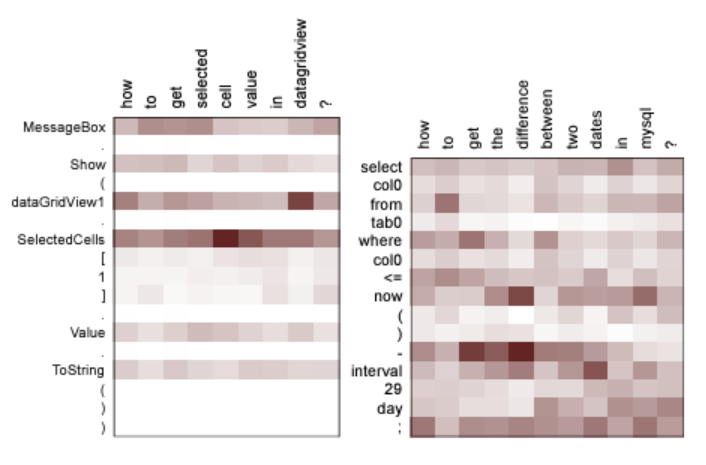
\includegraphics[width=0.8\textwidth]{img/codenn.png}
\end{exampleblock}
\end{frame}
\begin{frame}{Early approaches -- Supervised Learning}
\begin{exampleblock}{Malware Detection~\cite{DBLP:journals/tii/CuiXCCWC18}}
\centering
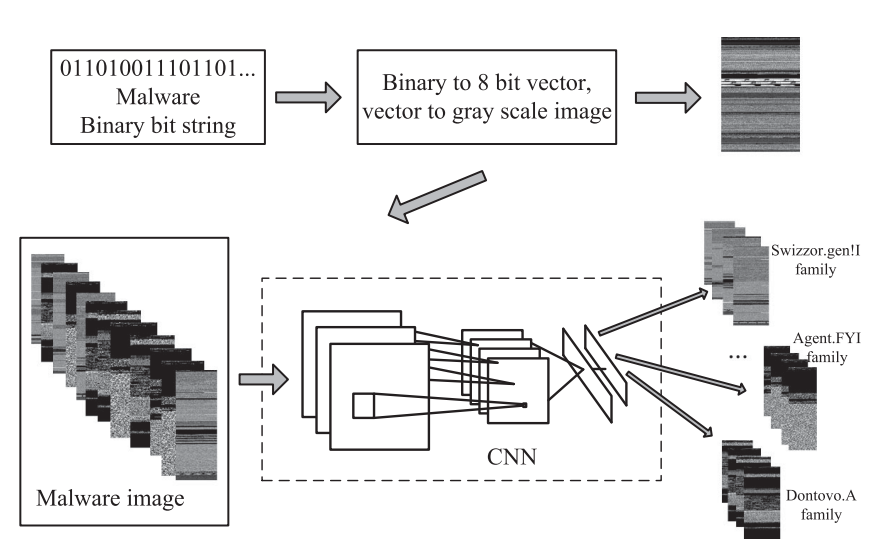
\includegraphics[width=0.8\textwidth]{img/malware-detection.png}
\end{exampleblock}
\end{frame}
\begin{frame}{Early approaches -- Supervised Learning}
\begin{exampleblock}{Code Review -- Deep Review~\cite{DBLP:conf/pakdd/LiSTHXLL19}}
\centering
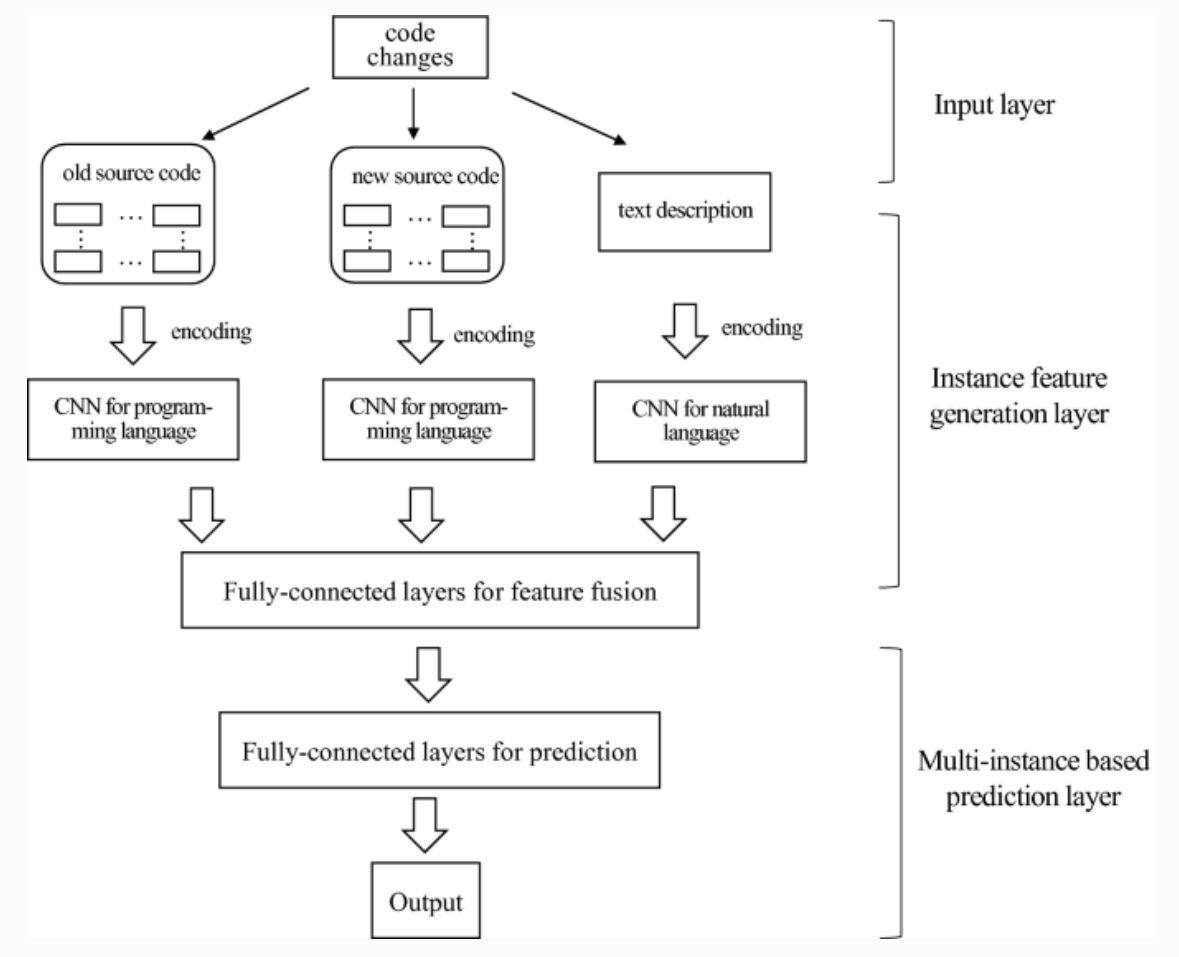
\includegraphics[width=0.6\textwidth]{img/deep-review.png}
\end{exampleblock}
\end{frame}
\begin{frame}{Early approaches -- Unsupervised Learning}
\begin{exampleblock}{Code Completion (kNN)~\cite{DBLP:conf/sigsoft/BruchMM09}}
\centering
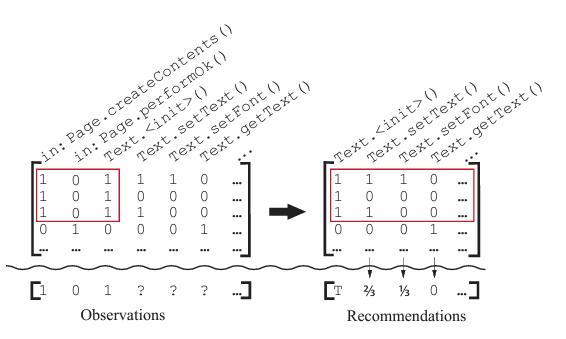
\includegraphics[width=0.8\textwidth]{img/code-completions.png}
\end{exampleblock}
\end{frame}
\begin{frame}{Early approaches -- Pitfalls}
	\begin{itemize}
		\item \textbf{Data scarcity:} software engineering data is scarce and expensive to collect, posing challenges for training effective models.
		\item \textbf{Single-task models:} many models are designed for \emph{specific} tasks, limiting their broader \emph{applicability} and \emph{reuse}.
		\item \textbf{Lack of generalization:} models often fail to \emph{generalize} across different software projects and domains.
		\item \textbf{Human-computer interaction:} Early models did not adequately consider human factors, impacting \emph{usability} and \emph{adoption} in software development practices.
	\end{itemize}
\end{frame}
\begin{frame}{Towards LLM solutions}
	\begin{exampleblock}{Why?}
		\begin{itemize}
			\item \textbf{Code understanding}: LLMs, correctly trained, can understand code and its context.
			\item \textbf{Code-Language link}: LLMs can link code to natural language, improving \emph{documentation} and \emph{understanding}.
			\item \textbf{Session support}: LLMs can support developers during coding sessions, providing \emph{hints} and \emph{suggestions}.
			\item \textbf{Testing support}: LLMs can generate \emph{test cases} and \emph{fault prediction}.
			\item \textbf{One-model-for-all}: LLMs can be used for \emph{multiple} tasks, reducing the need for \emph{task-specific} models.
			\item \textbf{Personalization}: LLMs can be personalized to the developer's \emph{style} and \emph{needs}.
			\item \textbf{Human-level performance}: LLMs can achieve human-level performance in \emph{specific} tasks.
		\end{itemize}
	\end{exampleblock}
\end{frame}
\begin{frame}[allowframebreaks]{LLM in SE -- Areas of Application}
	\begin{exampleblock}{Requirement Engineering}
			\begin{itemize}
					\item \textbf{Ambiguity Resolution}: enhancing clarity and understanding in requirements.
					\item \textbf{Requirement Classification}: categorizing requirements based on their nature and criticality.
					\item \textbf{Requirement Analysis}: in-depth analysis to ensure requirements are feasible, relevant, and comprehensive.
			\end{itemize}
	\end{exampleblock}
	
	\begin{exampleblock}{Software Development}
			\begin{itemize}
					\item \textbf{Code Generation}: automating the creation of code from specifications.
					\item \textbf{Code Summarization}: generating concise summaries of code blocks for easier understanding.
					\item \textbf{Code Completion}: predicting and providing code snippets to speed up development.
			\end{itemize}
	\end{exampleblock}

	\framebreak

	\begin{exampleblock}{Software Quality}
			\begin{itemize}
					\item \textbf{Test Generation}: audiotomatically creating tests to validate software functionality.
					\item \textbf{Fault Prediction}: identifying potential areas of the codebase that are prone to errors.
					\item \textbf{Bug Localization}: pinpointing the exact location of bugs in the codebase.
					\item \textbf{API Documentation}: generating comprehensive documentation for APIs.
			\end{itemize}
	\end{exampleblock}

	\begin{exampleblock}{Software Maintenance}
			\begin{itemize}
					\item \textbf{Code Review}: automating the review process to identify potential issues.
					\item \textbf{Bug Prediction}: forecasting bugs in future iterations based on historical data.
					\item \textbf{Refactoring}: suggesting code improvements for better maintainability and performance.
					\item \textbf{Commit Classification}: categorizing commits for better project tracking and management.
			\end{itemize}
	\end{exampleblock}
\end{frame}
\begin{frame}{LLM for SE -- How?}
Three main layers:
\begin{itemize}
	\item \textbf{Foundational models}: LLMs trained on a large corpus of text, it can contains code.
	\begin{itemize}
		\item GPT, Llama, Mistral, etc.
	\end{itemize}
	\item \textbf{Fine-tuned models}: LLMs can be fine-tuned using specific instruction/dataset
	\begin{itemize}
		\item Codex, CodeLlama, etc.
	\end{itemize}
	\item \textbf{Adaptation layer}: LLMs can be adapted to specific tasks using \emph{prompting} and other techniques.
	\begin{itemize}
		\item Copilot, MetaGPT, etc.
	\end{itemize}
\end{itemize}
\end{frame}
\begin{frame}[allowframebreaks]{Prompt-engineering}
\begin{exampleblock}{Zero Shot~\cite{DBLP:conf/iclr/WeiBZGYLDDL22}}
	\textbf{Technique:} Direct instruction for desired outcome without fine-tuning. \\
	\emph{Example:} "Translate the following text into French: 'Hello, how are you?'"
\end{exampleblock}
\begin{exampleblock}{Few-Shot Learning~\cite{DBLP:conf/nips/BrownMRSKDNSSAA20}}
	\textbf{Technique:} Use minimal examples in prompt for in-context learning. \\
	\emph{Example:} "Given a sentence identify the subject and the action.

	Examples:
	1. ’The dog barked loudly.’ Subject: dog, Action: barked
	2. ’The leaves fell from the tree.’ Subject: leaves, Action: fell
	
	Now, identify the subject and the action in the sentence: ’The cat meowed loudly.’"
\end{exampleblock}

\begin{columns}
\begin{column}{0.75\textwidth}
	\begin{exampleblock}{Chain of thought~\cite{DBLP:conf/nips/Wei0SBIXCLZ22}}
		\textbf{Technique:} Break down a complex problem into smaller steps. \\
		\emph{Example:} "To calculate the total cost, first find the cost per item, then multiply by the number of items."
		\end{exampleblock}
\end{column}
\begin{column}{0.2\textwidth}
	\centering
	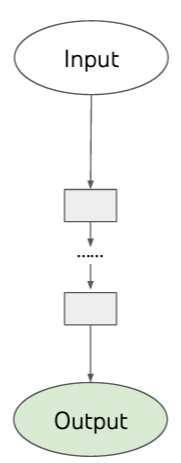
\includegraphics[width=\textwidth]{img/cot.png}	
\end{column}
\end{columns}
\framebreak

\begin{exampleblock}{Self-consistency}
\textbf{Technique:} Sampling \emph{multiple}, \emph{diverse} reasoning paths through few-shot CoT, and use the generations to select the \emph{most} consistent answer 
\emph{Example:} "
Q: Today I have 6 apples. Tomorrow I buy 3 more. How many apples do I have?\\
A: 9\\
Q: Today I have 6 apples. Yesterday I ate 6 apples, How many apples do I have?\\
A: 6\\
Q: Today I have 6 apples. Tomorrow I buy 3 more. Yesterday I ate 6 apples, How many apples do I have? \\
"\\
Answers: 6, 6, 9 => the model selects 6
\end{exampleblock}

\begin{columns}
	\begin{column}{0.6\textwidth}
		\begin{exampleblock}{Tree of thought}
			\textbf{Technique:} Explore multiple reasoning paths for comprehensive analysis. \\
			\emph{Example:} "Imagine three different experts are answering this question.
			All experts will write down 1 step of their thinking,
			then share it with the group.
			Then all experts will go on to the next step, etc.
			If any expert realises they're wrong at any point then they leave.
			The question is..."
			\end{exampleblock}
	\end{column}
	\begin{column}{0.35\textwidth}
	
		\centering
		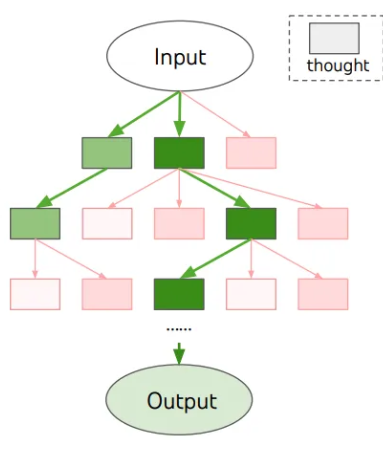
\includegraphics[width=\textwidth]{img/toc.png}	
	\end{column}
\end{columns}
\begin{exampleblock}{Retrieval Augmented Generation (RAG)}
	\textbf{Technique:} Leverages \emph{external} knowledge by \emph{retrieving} relevant documents and then generating an answer based on both the prompt and the retrieved documents. \\
	\emph{Example:} "Q: Who was the president of the United States in 1955?\\
	
	R: << add local embedding >> 
	
	A: 'Dwight D. Eisenhower'
	\end{exampleblock}
	\centering
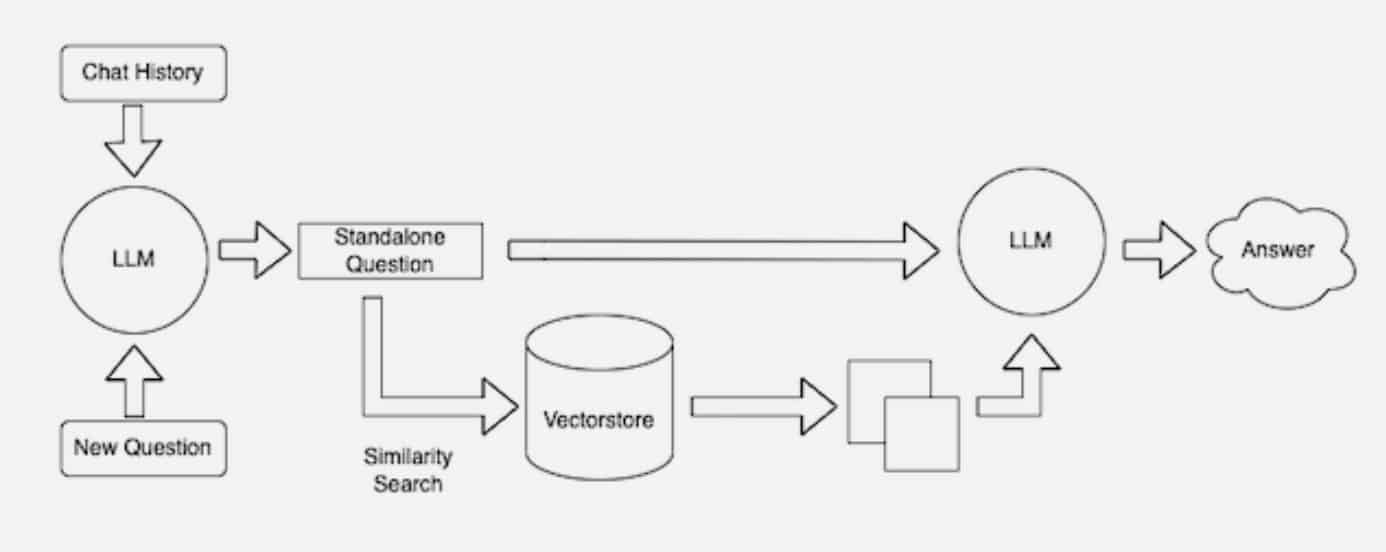
\includegraphics[width=0.8\textwidth]{img/rag.jpg}

\begin{exampleblock}{Progressive refinement}
	\textbf{Technique:} Refine the response through iterative prompting. \\
	\emph{Example:} Initial prompt: "What factors influence climate change?" Follow-up: "How do carbon emissions affect these factors?"
	\end{exampleblock}
\begin{exampleblock}{Role play}
\textbf{Technique:} Assign a specific perspective or character to the model. \\
\emph{Example:} "As a nutritionist, list the benefits of a plant-based diet."
\end{exampleblock}
\begin{exampleblock}{ReAct~\cite{yao2022react}}
\textbf{Technique:} Combines reasoning and action to create smarter, context-aware prompts by leveraging LLMs for generating reasoning traces and task-specific actions in an interleaved manner. \\
\emph{Example}: 
"Q: What is the capital of France?\\
T-1: I need to find the capital city of France.\\
A-1: Search[capital of France]\\
O-1: The capital of France is Paris.\\
T-2: The capital city of France is identified as Paris.\\
A-2: Finish[Paris]
"
\end{exampleblock}
\end{frame}
\begin{frame}{Interact with LLM}
	\begin{itemize}
		\item Via direct API: using the \emph{API} of the model. 
		\begin{itemize}
			\item \faThumbsUp: full access to the model, it can be also fine tuned;
			\item \faThumbsDown: sometimes you do not have access to model weights (e.g., GPT-3);
			\item \faThumbsDown: sometimes even if the model is open, it is too \emph{big} to be used in a local environment (e.g., Falcon 180b).
		\end{itemize}
		\item Via HTTP API: using a \emph{web service} that wraps the model.
		\begin{itemize}
			\item OpenAI as reference\footnote{\url{https://platform.openai.com/}}
			\item \faThumbsUp: easy to use;
			\item \faThumbsUp: can be used in \emph{any} environment.
			\item \faThumbsUp: can also be used with \emph{local}
			models (e.g., ollama)
		\end{itemize}
	\end{itemize}
\end{frame}
\begin{frame}{Ollama}
\begin{center}

\includegraphics[width=0.2\textwidth]{img/ollama.png}\\
\url{https://ollama.com/}
\end{center}
\begin{itemize}
	\item A platform that wraps LLMs in a web service.
	\begin{itemize}
		\item More than 60 models available.
		\item Allow customizing the model.
		\item Native performance for LLMs.
	\end{itemize}
\end{itemize}
\begin{itemize}
	\item How to use?
	\begin{itemize}
		\item Pull a model: \texttt{ollama pul llama2}
		\item Use the model: \texttt{ollama run llama2}
		\item Start a web service: \texttt{ollama serve}
		\end{itemize}
\end{itemize}
\end{frame}

\begin{frame}{LangChain}
\begin{center}

\includegraphics[width=0.5\textwidth]{img/logo.png}
\url{https://github.com/langchain-ai/langchain}
\end{center}
\begin{itemize}
	\item A framework for developing applications powered by language models.
	\item Features:	
	\begin{itemize}
		\item Support several API providers (e.g., OpenAI, Ollama, etc.)
		\item Support the combination of several processing steps (e.g., prompting, chaining, etc.)
		\item Support the context retrivial (e.g., RAG)
	\end{itemize}
\end{itemize}
\begin{center}
\huge{\textbf{Demo}}
\url{https://github.com/cric96/langchain-examples}
\end{center}
\end{frame}
\begin{frame}{Software Development -- Current Tools}
\begin{exampleblock}{Desing guiding principles}
	\begin{itemize}
		\item \textbf{IDE-integrated:} seamless integration in IDEs.
		\item \textbf{Agility:} Support for quick iterations and adaptability.
		\item \textbf{Chat-oriented:} conversational interfaces for fast interactions.
	\end{itemize}
\end{exampleblock}
\begin{exampleblock}{State-of-the-art solutions}
	\begin{itemize}
		\item \textbf{Copilot X} \url{https://github.com/features/copilot}
		\begin{itemize}
			\item The standard de-facto for code generation / code completion, providing context-aware suggestions to streamline coding tasks.
		\end{itemize}
		\item \textbf{CodeWhisper} \url{https://aws.amazon.com/it/codewhisperer/features/}
		\begin{itemize}
			\item An AI-powered pair programmer from Amazon.
		\end{itemize}
		\item \textbf{Continue}: \url{https://continue.dev/docs/how-to-use-continue}
		\begin{itemize}
			\item Leverage LLMs (open and closed) to provide \emph{hints} and \emph{suggestions} during coding sessions.
		\end{itemize}
	\end{itemize}
\end{exampleblock}
\end{frame}
\begin{frame}{Copilot X}
\begin{center}

\includegraphics[width=0.2\textwidth]{img/copilot-logo.png}

\url{https://github.com/features/copilot}
\end{center}

\begin{itemize}
	\item Solution developed by Microsoft specialized for code development
	\item Released in 2021, now it has more than 1 million users.
	\item Integrated in several IDEs
	\begin{itemize}
		\item Visual Studio Code
		\item IntelliJ
	\end{itemize}
\end{itemize}
\end{frame}
\begin{frame}{Copilot X -- Report\footnote{\url{https://github.blog/2022-09-07-research-quantifying-github-copilots-impact-on-developer-productivity-and-happiness/}}}
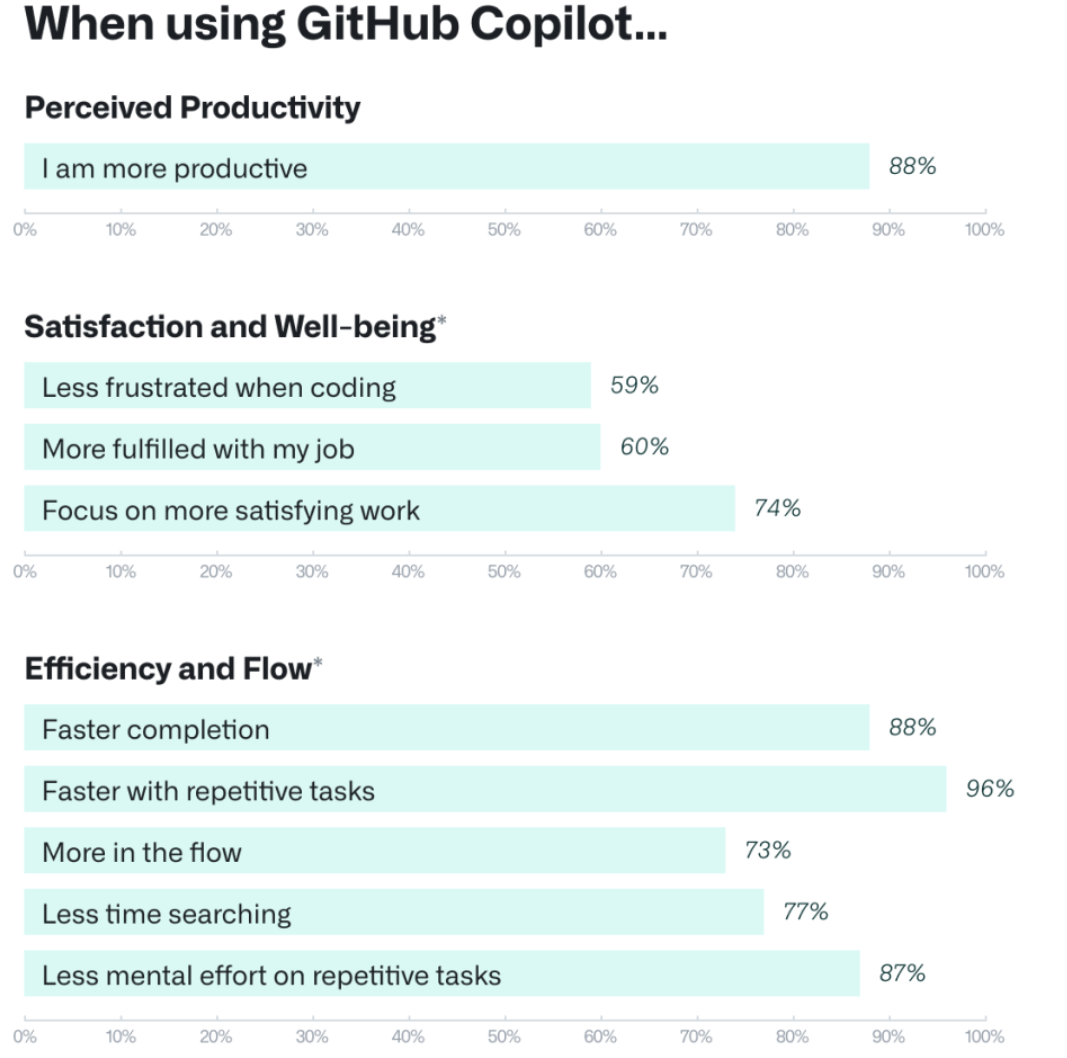
\includegraphics[width=0.35\textwidth]{img/copilot-report-1.png}
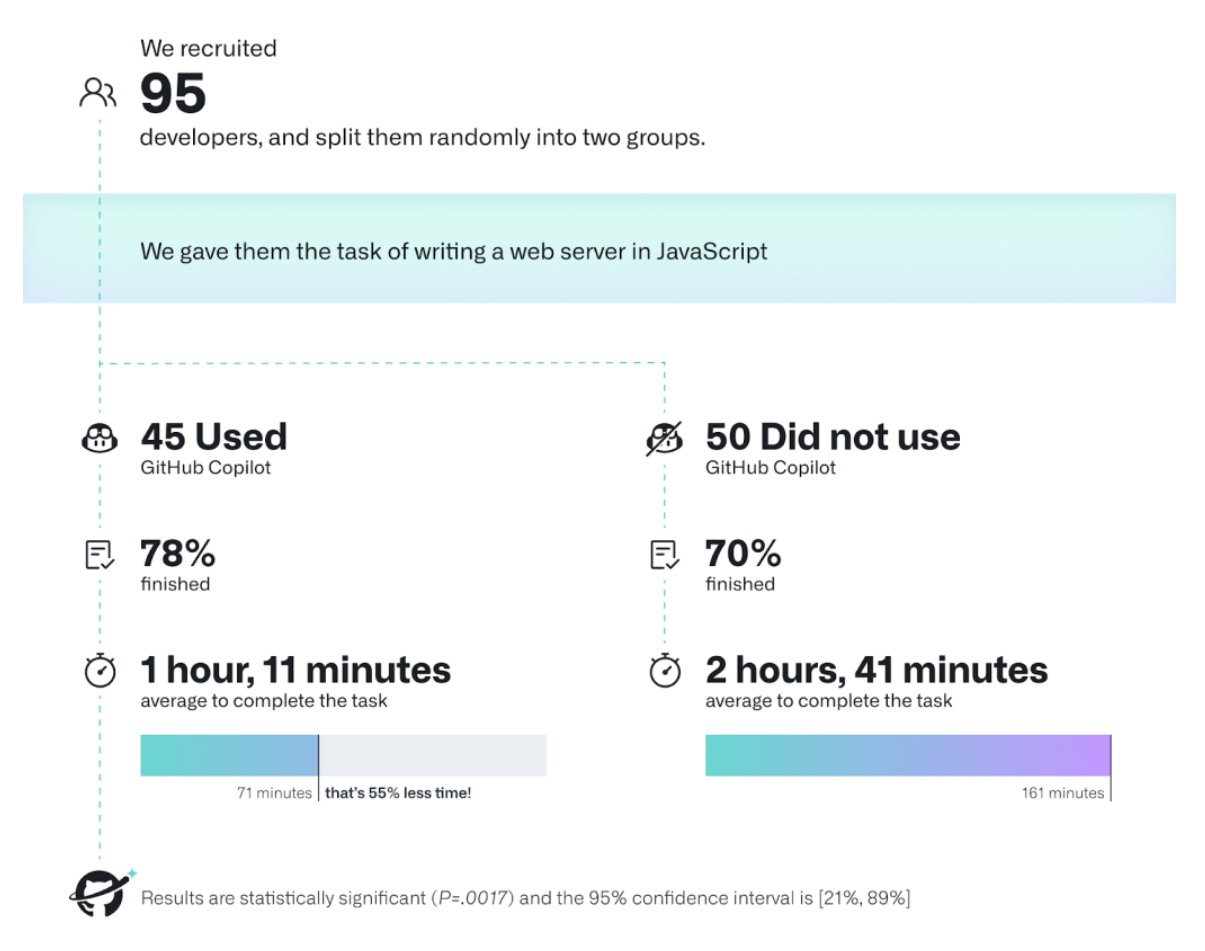
\includegraphics[width=0.55\textwidth]{img/copilot-report-2.png}
\end{frame}
\begin{frame}{Copilot X Concerns -- Security\footnote{\url{https://blog.gitguardian.com/yes-github-copilot-can-leak-secrets/}}}

\includegraphics[width=\textwidth]{img/copilot-concerns.png}
\end{frame}
\begin{frame}{Copilot X Concerns -- Code Quality\footnote{\url{https://www.gitclear.com/coding_on_copilot_data_shows_ais_downward_pressure_on_code_quality}}}
	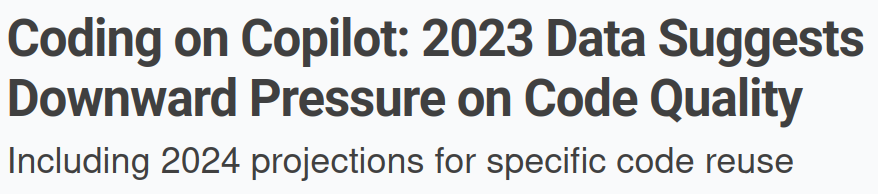
\includegraphics[width=\textwidth]{img/problem-code-quality.png}
	\end{frame}
\section{LLMs for Software Testing}
\begin{frame}{LLMs for Software Testing~\cite{wang2024software}}
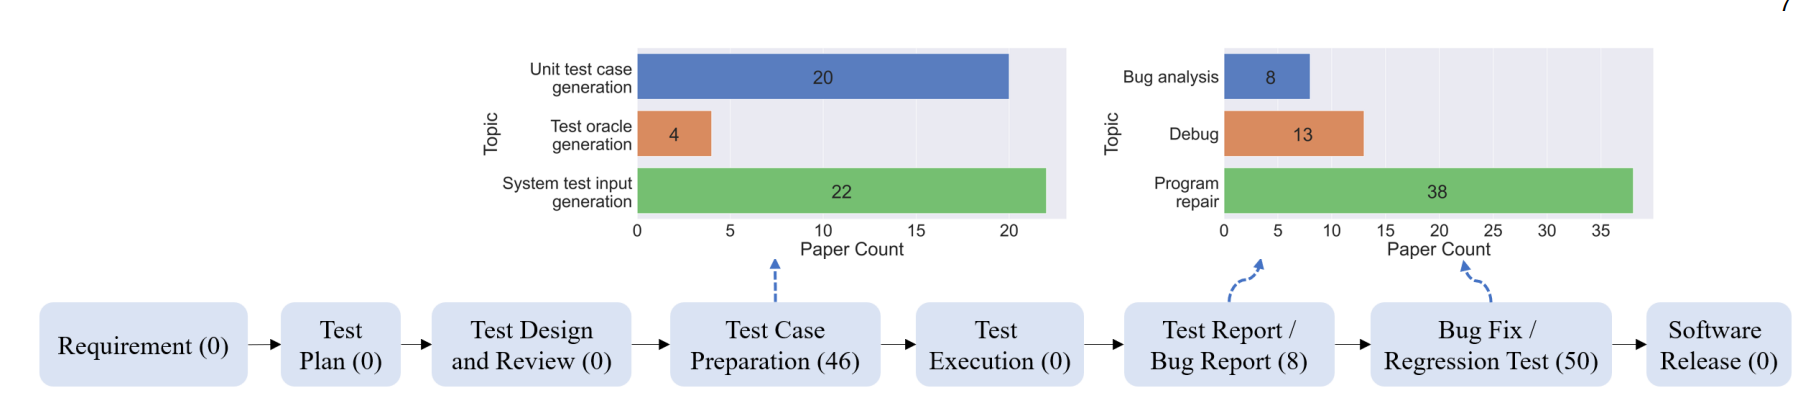
\includegraphics[width=\textwidth]{img/overview.png}
\begin{itemize}
	\item Takeaways:
	\begin{itemize}
		\item LLMs can be used for \emph{multiple} testing tasks.
		\item Currently, LLMs are used for \emph{test case generation} and \emph{bug fix}.
	\end{itemize}
\end{itemize}
\end{frame}
\begin{frame}{LLMs for Software Testing -- Methods}
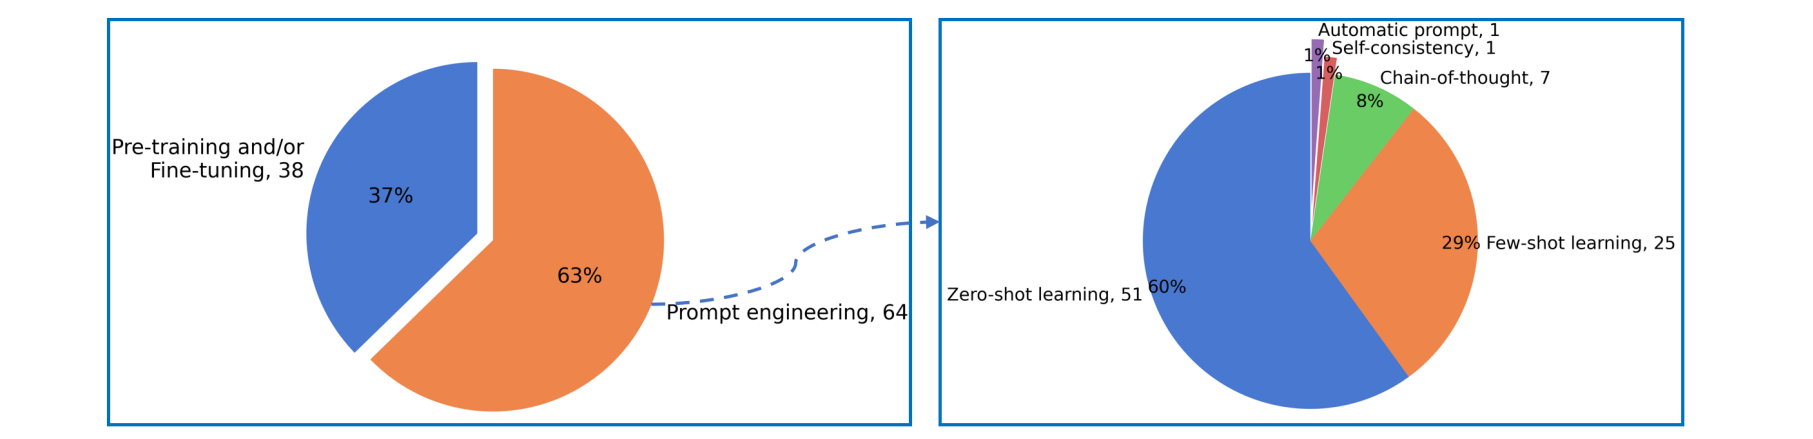
\includegraphics[width=\textwidth]{img/how-llm-are-used.png}
\begin{itemize}
	\item Takeaways:
	\begin{itemize}
		\item Prompt Engineering is the main method used to adapt LLMs to testing tasks.
		\begin{itemize}
			\item Why? No need to fine-tune the model.
			\item Why? Can be used with any LLM.
		\end{itemize}
		\item \textbf{Zero-shot learning} is the most used method.
		\begin{itemize}
			\item Simple and effective.
			\item Concerns about its effectiveness.
		\end{itemize}
	\end{itemize}
\end{itemize}
\end{frame}
\begin{frame}{LLMs for Software Testing -- Methods}
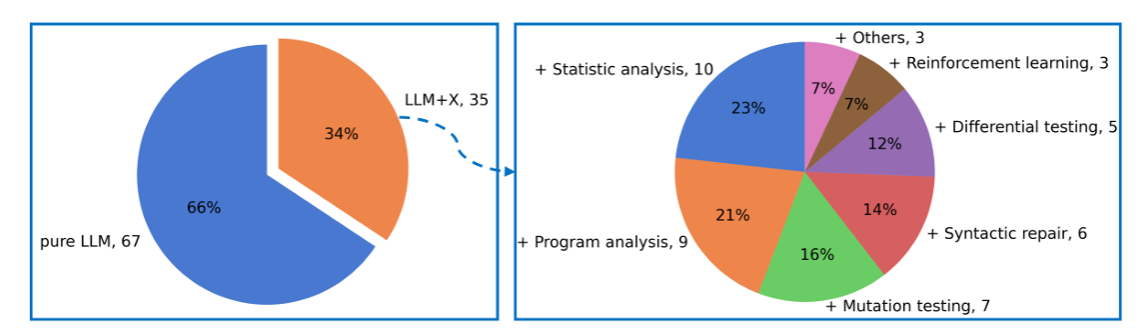
\includegraphics[width=\textwidth]{img/llm-usage.png}
\begin{itemize}
	\item Modern solution integrate LLM in standard testing tools.
	\begin{itemize}
		\item LLM used as an \emph{intelligent} agent in the testing process -- more example will be shown in the next slides.
	\end{itemize}
\end{itemize}
\end{frame}
\begin{frame}{LLMs for Software Testing -- Input}
\centering
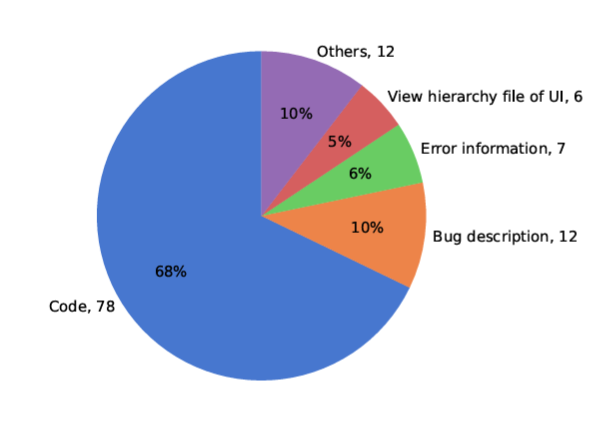
\includegraphics[width=0.5\textwidth]{img/input-llm.png}
\begin{itemize}
	\item Takeaways:
	\begin{itemize}
		\item Passing the code as input is the most used method.
		\item Additional information seems to be useful.
	\end{itemize}
\end{itemize}
\end{frame}
\section{Innovative Solutions for LLMs -- LLM-Agent models}
\begin{frame}[plain]
\centering
\huge{LLM-Agent-Based Architectures}
\large{ 
Complex archictures that leverage LLMs to create autonomous agents that can interact with the \emph{environment} and other LLM-agents.
}
\end{frame}
\begin{frame}{LLM-Agent -- Overview~\cite{wang2023survey}}
	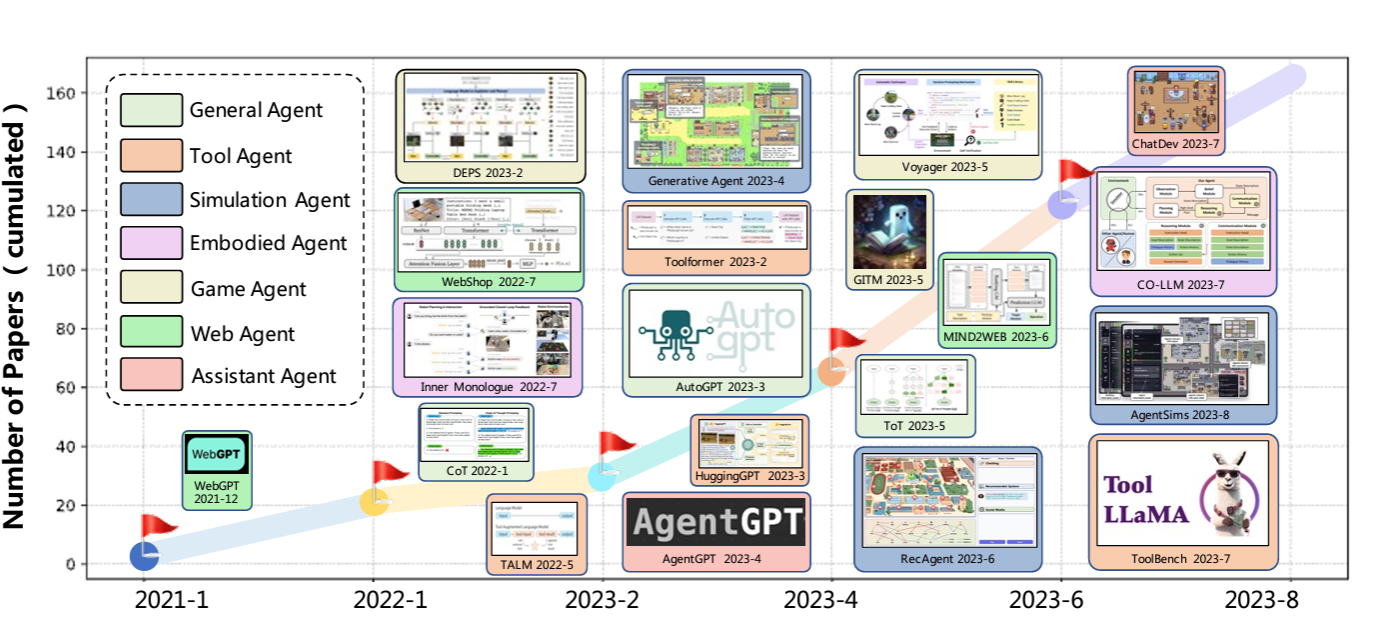
\includegraphics[width=\textwidth]{img/number-of-papers.png}
\end{frame}
\begin{frame}{LLM-Agent -- Modules}
	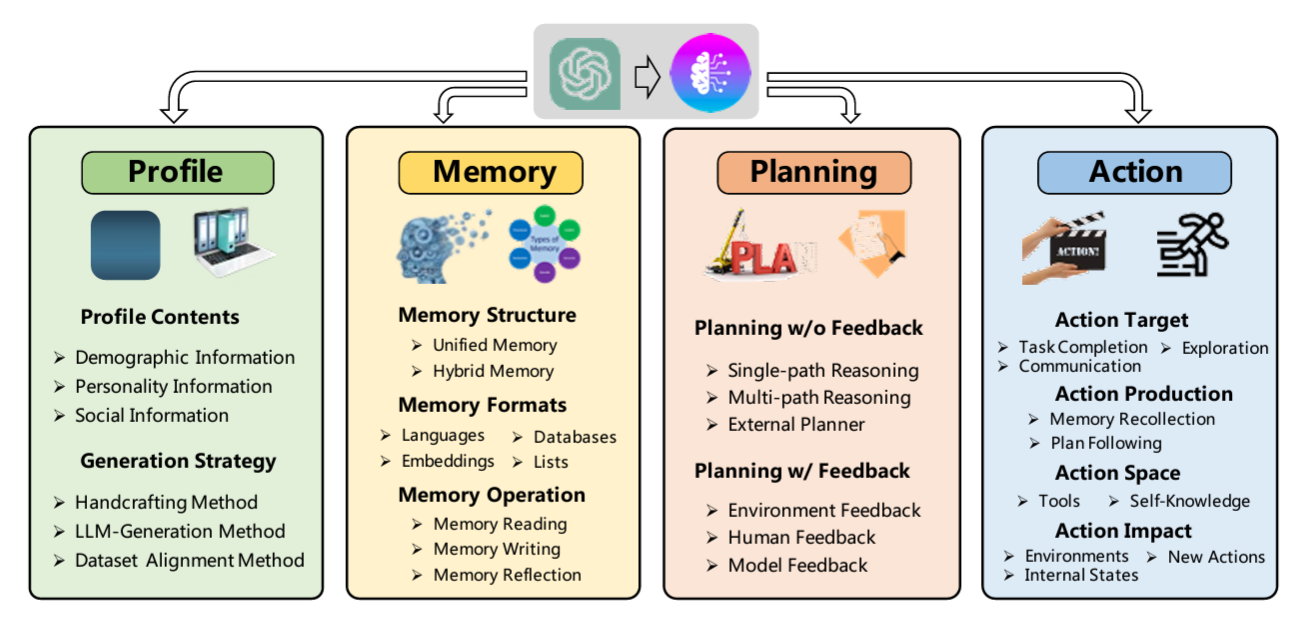
\includegraphics[width=\textwidth]{img/overview-agents.png}
\end{frame}
\begin{frame}{Meta GPT~\cite{hong2023metagpt}}
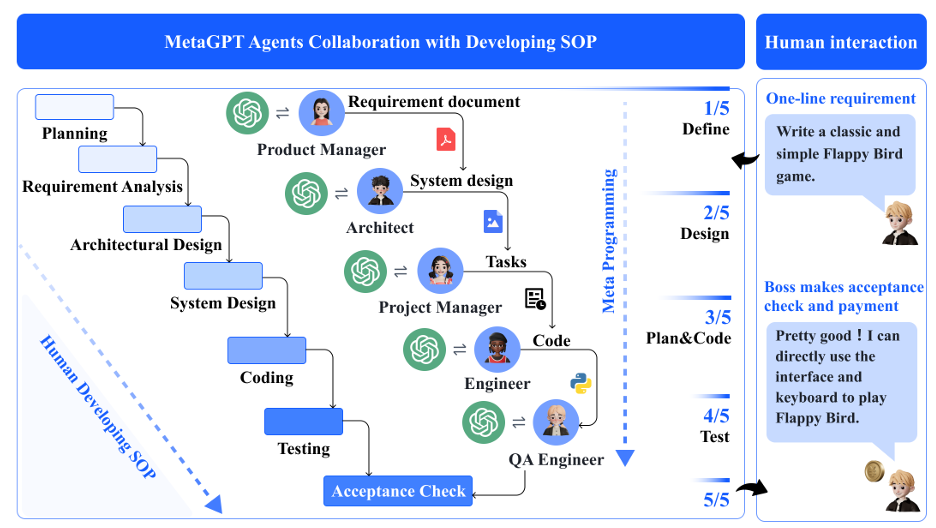
\includegraphics[width=\textwidth]{img/meta-gpt-idea.png}
\end{frame}
\begin{frame}{Auto GPT~\footnote{\url{https://github.com/Significant-Gravitas/AutoGPT}}}
	\centering
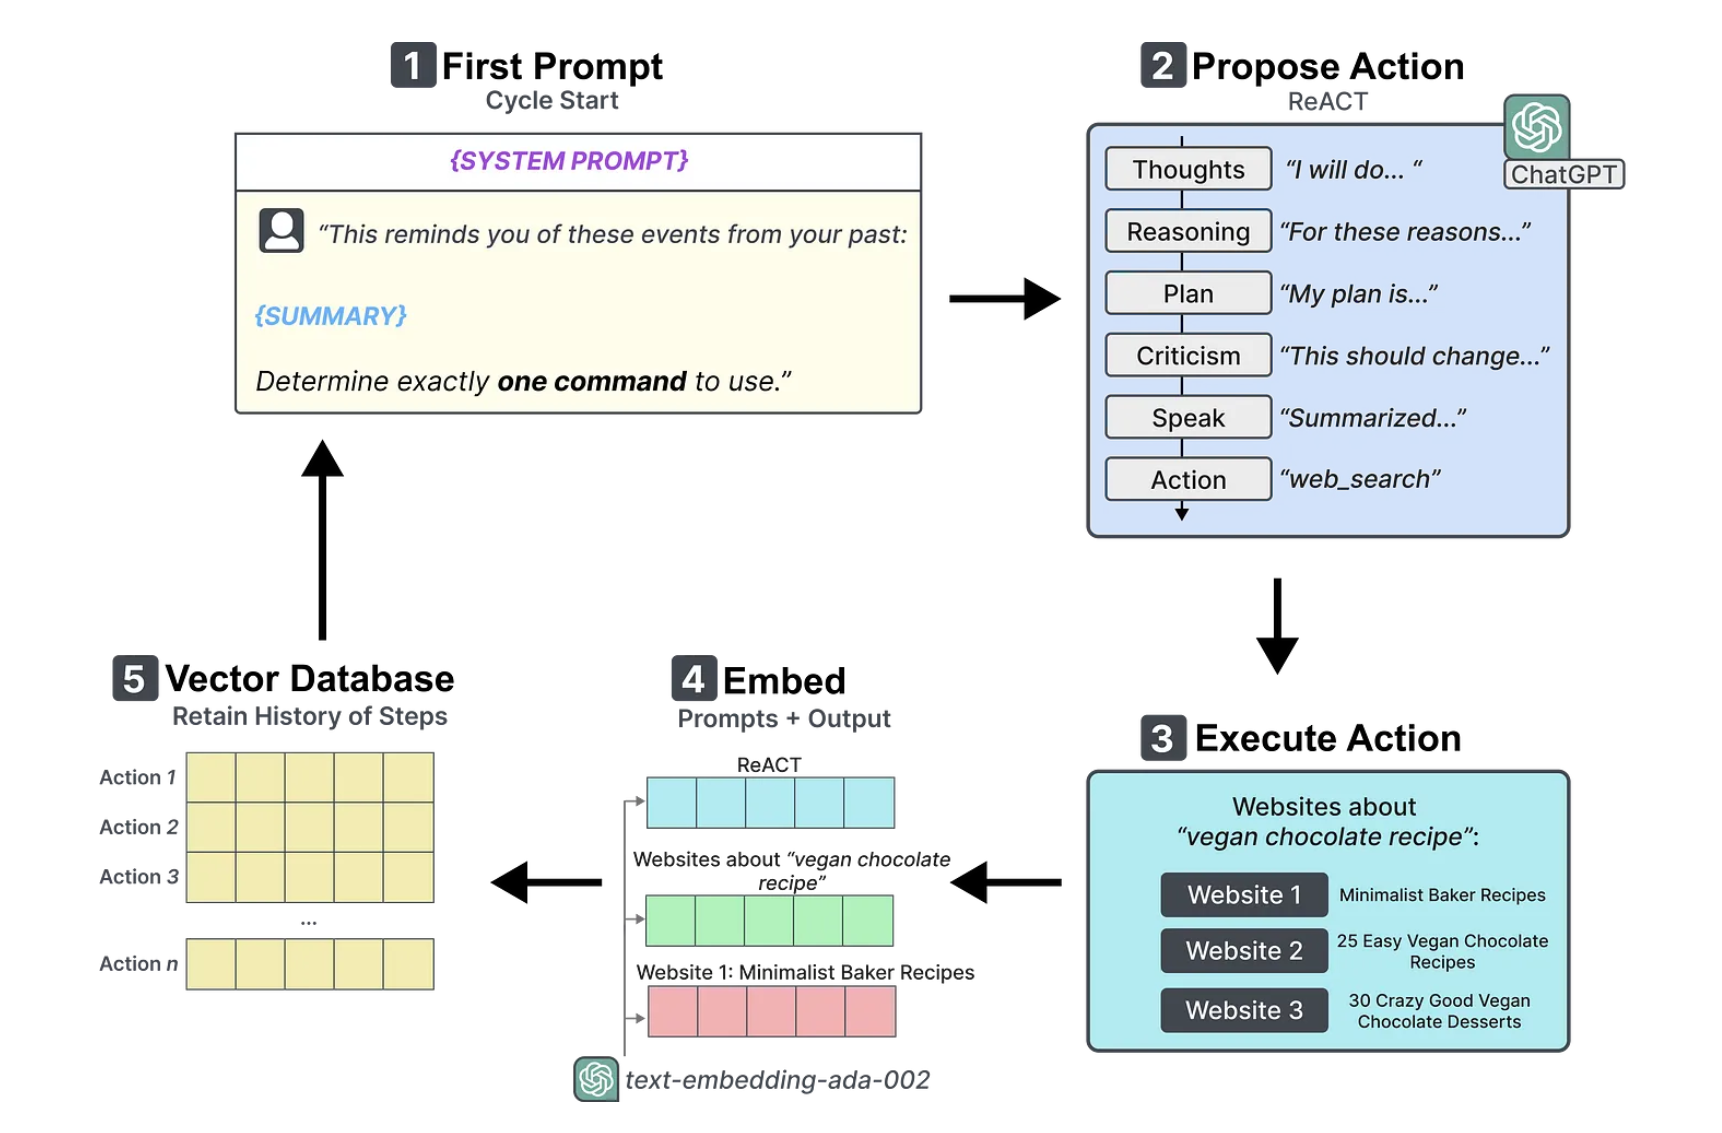
\includegraphics[width=0.9\textwidth]{img/auto-gpt-loop.png}
\end{frame}
\begin{frame}{AgentVerse~\cite{chen2023agentverse}}
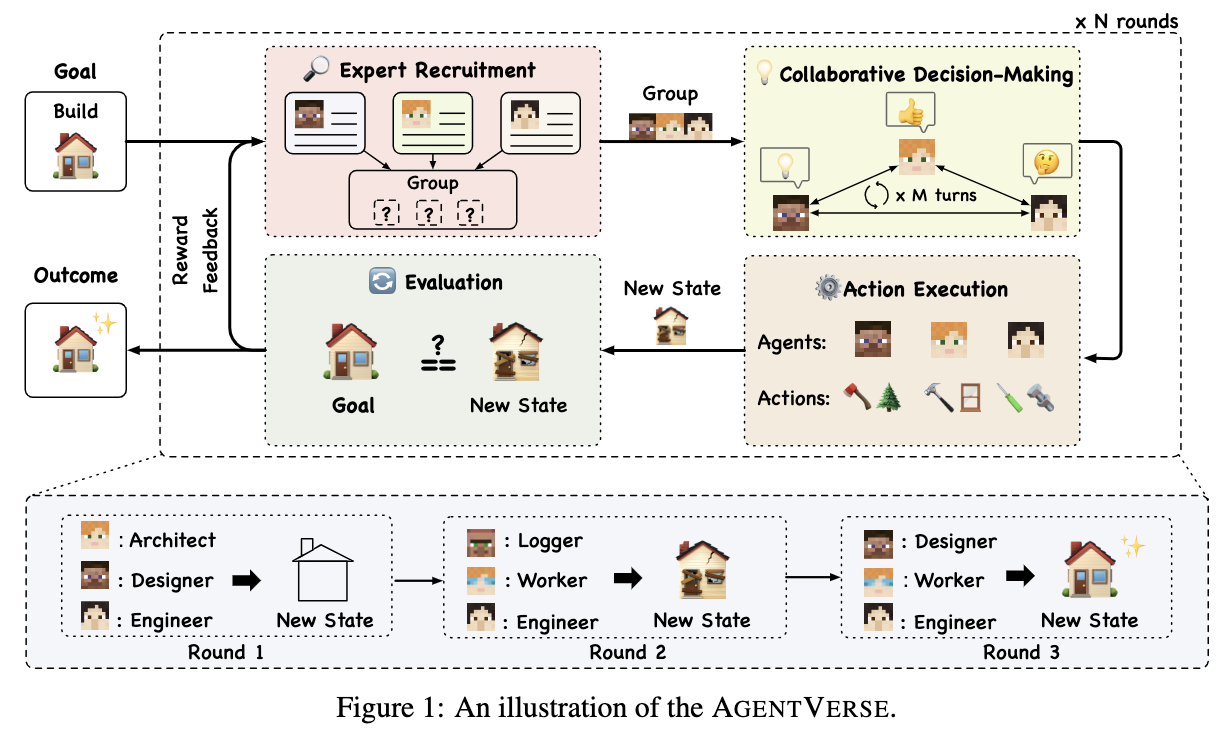
\includegraphics[width=\textwidth]{img/agent-verse.png}
\end{frame}
\begin{frame}{Conclusion}
	\centering

\includegraphics[width=0.8\textwidth]{img/king-of-all-the-king.png}
\end{frame}
\begin{frame}{Conclusion -- Seriously}
\begin{itemize}
	\item ML in SE is a long-standing research area.
	\item LLMs are a \emph{game changer} in this context.
	\item LLMs can be applied to \emph{multiple} SE tasks.
	\begin{itemize}
		\item \emph{Code generation}, \emph{testing}, \emph{requirement engineering}, etc.
	\end{itemize}
	\item Novel paradigm:
	\begin{itemize}
		\item \emph{One-model-for-all} approach.
		\item \emph{Personalization} of the model.
		\item \emph{Adaptation} of the model to specific tasks.
		\item Advanced solutions for making the LLM \emph{autonomous}.
	\end{itemize}
\end{itemize}
\end{frame}
%===============================================================================

%/////////
\frame{\titlepage}
%/////////

%===============================================================================
\section*{\refname}
%===============================================================================

%%%%
\setbeamertemplate{page number in head/foot}{}
%/////////
\begin{frame}[c,noframenumbering, allowframebreaks]{\refname}
%\begin{frame}[t,allowframebreaks,noframenumbering]{\refname}
	\tiny
	\printbibliography
\end{frame}
%/////////

%%%%%%%%%%%%%%%%%%%%%%%%%%%%%%%%%%%%%%%%%%%%%%%%%%%%%%%%%%%%%%%%%%%%%%%%%%%%%%%%
\end{document}
%%%%%%%%%%%%%%%%%%%%%%%%%%%%%%%%%%%%%%%%%%%%%%%%%%%%%%%%%%%%%%%%%%%%%%%%%%%%%%%%
